% ═══════════════════════════════════════════════════════════════════
% An Asymmetric Dimensional Barrier in Causal-Set Link Dynamics
% Selects 3+1 Dimensions
% Author: Gang Zhang
% Date: March 2026
% Version: 1.5
% ═══════════════════════════════════════════════════════════════════
\documentclass[12pt,a4paper]{article}

% ── Packages ────────────────────────────────────────────────────────
\usepackage[utf8]{inputenc}
\usepackage[T1]{fontenc}
\usepackage{lmodern}
\usepackage{amsmath,amssymb,amsfonts}
\usepackage{graphicx}
\usepackage{booktabs}
\usepackage{hyperref}
\usepackage[margin=2.5cm]{geometry}
\usepackage{enumitem}
\usepackage{caption}
\usepackage{float}
\usepackage{xcolor}
\usepackage{setspace}
\usepackage[numbers,sort&compress]{natbib}
\usepackage{listings}

\bibliographystyle{unsrtnat}

\hypersetup{
    colorlinks=true,
    linkcolor=blue!70!black,
    citecolor=blue!70!black,
    urlcolor=blue!70!black,
}

\graphicspath{{figures/}}

% ── Title ───────────────────────────────────────────────────────────
\title{An Asymmetric Dimensional Barrier in Causal-Set Link Dynamics\\
Selects 3+1 Dimensions}

\author{Gang Zhang\thanks{Email: unicome@gmail.com}\\
\small Independent Researcher}
\date{March 2026}

% ════════════════════════════════════════════════════════════════════
\begin{document}
\setstretch{1.15}
\maketitle

% ── Abstract ────────────────────────────────────────────────────────
\begin{abstract}
We study the dimensional-selection problem in a finite ensemble of discrete causal partial orders (posets).
Each poset is assigned a statistical weight through an effective action balancing combinatorial entropy
against a causal-dynamical penalty term.
We compare Lorentzian-like families sprinkled into 2, 3, 4, and 5 flat spacetime dimensions.

We find that the dimensional-selection signal in causal-set link dynamics is not characterized by a
fixed parameter window, which shifts under changes of generator geometry, but by a nearly
generator-independent critical control ratio.
A \textbf{link-based causal action} --- the $d=2$ Benincasa--Dowker action $S = N - 2C_0$ ---
exhibits a $3{+}1$-dimensional selection window whose location in coupling space varies across generators,
but whose underlying control structure does not.

In contrast, the \textbf{standard $d=4$ BDG action}
$S^{(4)} = N - C_0 + 9C_1 - 16C_2 + 8C_3$ systematically selects 5D at every coupling and every size
tested: the higher-order interval corrections destroy dimensional selection by preferentially favoring
causally sparse, high-dimensional configurations.

The key result is the identification of a dimensionless control parameter
$\Xi_{d \to d+1}$ --- the link-penalty separation per unit entropy separation between adjacent dimensions.
The $4{\to}5$ boundary occurs at $\Xi_{4 \to 5} \approx 10$ across all three generators tested
(cube sprinkle, independent-seed cube, and Alexandrov-set diamond; coefficient of variation $13.9\%$),
substantially larger than the corresponding lower-dimensional thresholds
($\Xi_{3 \to 4} \approx 2{-}5$, $\Xi_{2 \to 3} \approx 1{-}3$).
Blind extrapolation to higher dimensions yields measured values
$\Xi_{5 \to 6} \approx 46$ and $\Xi_{6 \to 7} \approx 38$,
confirming that barriers intensify dramatically beyond 4D.
This asymmetric barrier structure makes $3{+}1$ dimensions a \textbf{natural equilibrium point} of the
entropy--connectivity competition: the link-penalty cost of ascending from 4D to 5D is an order of
magnitude steeper, per unit entropy gained, than any lower-dimensional transition.
It is not 4D itself that is special, but the barrier above it.
\end{abstract}

\tableofcontents
\newpage

% ════════════════════════════════════════════════════════════════════
\section{Introduction}
\label{sec:introduction}

\subsection{The Dimensionality Problem}
\label{sec:dim_problem}

Why observed macroscopic spacetime has $3{+}1$ effective dimensions remains one of the deepest open
problems in fundamental physics.
In many approaches --- string theory, Kaluza--Klein, large extra dimensions --- the answer is displaced
rather than derived: extra dimensions are postulated and later compactified or hidden.
A more fundamental question is:

\begin{quote}
Can a $3{+}1$-dimensional Lorentzian-like phase emerge as the structurally favored candidate inside a
broader discrete causal space, without being inserted by hand?
\end{quote}

\subsection{Causal Set Theory and the BDG Action}
\label{sec:causal_set}

Causal set theory \cite{Bombelli1987,Surya2019} provides one of the most natural frameworks for this
question. A causal set is a locally finite partially ordered set whose order relation encodes the causal
structure of spacetime. The Benincasa--Dowker--Glaser (BDG) action \cite{Benincasa2010} provides a
discrete analogue of the Einstein--Hilbert action:
\begin{equation}
S^{(d)}_\text{BDG} = \sum_{k=0}^{d/2} \alpha_k^{(d)} \, C_k
\label{eq:bdg_general}
\end{equation}
where $C_k$ counts the number of order-$k$ causal intervals (pairs of elements with exactly $k$ elements
between them), and $\alpha_k^{(d)}$ are dimension-dependent coefficients derived from continuum matching.
For $d=2$:
\begin{equation}
S^{(2)}_\text{BDG} = S_\text{link} = N - 2C_0
\label{eq:link_action}
\end{equation}
which we call the \emph{link action}: it counts only elements and direct links (covering relations).
For $d=4$:
\begin{equation}
S^{(4)}_\text{BDG} = N - C_0 + 9C_1 - 16C_2 + 8C_3
\label{eq:bdg_d4}
\end{equation}
with additional higher-order interval terms designed to recover the scalar curvature in the continuum limit \cite{Glaser2018}.

\subsection{Summary of Results}
\label{sec:summary_results}

We report seven principal results, organized in order of logical dependence:

\begin{enumerate}[label=\textbf{R\arabic*}.]
\item \textbf{The link action selects 4D.}
  In a score function $\mathrm{Score}(G;\lambda) = -\beta \cdot H(G) + \lambda \cdot S(G)/N$,
  the link action produces a $\lambda$-window ($\lambda \approx 6{-}8$) where 4D families
  consistently outscore 2D, 3D, and 5D. The 4D selection is stable across $N = 20{-}68$
  (Section~\ref{sec:link_action_results}).

\item \textbf{The 4D selection extends to $N = 112$.}
  Large-$N$ experiments confirm that 4D wins at $\lambda = 10$ up through $N = 112$,
  with the selection window shifting to higher $\lambda$ at $N \geq 96$.
  A link-density crossover at $N \approx 96$ (3D surpasses 4D in link density)
  provides a mechanistic explanation for the finite-size window shift
  (Section~\ref{sec:large_n}).

\item \textbf{The standard BDG $d{=}4$ action selects 5D.}
  With literature coefficients, the BDG action systematically picks 5D at
  every coupling, for all sizes $N = 20{-}68$, and across all tested generators.
  Component analysis shows that the $C_1$--$C_3$ correction terms amplify
  the entropy advantage of 5D, destroying the link action's dimensional barrier
  (Section~\ref{sec:bdg_failure}).

\item \textbf{The $\Xi$ parameter identifies the structural origin.}
  We define a dimensionless control variable
  $\Xi_{d \to d+1} = |\Delta \bar S| / |\Delta \bar h|$
  measuring the link-action separation per unit entropy separation.
  $\Xi_{4\to5} \approx 10$ is stable across three generators (CV~$= 13.9\%$)
  and across sizes from $N = 20$ to $N = 112$ (CV~$= 17.7\%$)
  (Section~\ref{sec:xi_parameter}).

\item \textbf{Analytical derivation: $\Xi_{4 \to 5} = 11.8$.}
  From empirical scaling laws of $C_0/N$ and $\log H/N$, we derive a
  closed-form expression that yields $\Xi_{4\to5} = 11.8$, within $17\%$
  of the numerical median. The root cause is entropy saturation
  ($\Delta b_{4\to5}$ is $38\%$ of $\Delta b_{3\to4}$) combined with
  link-density gap persistence ($7.3\times$ larger at the $4{\to}5$ boundary)
  (Section~\ref{sec:xi_derivation}).

\item \textbf{Predictive validation: $d \geq 6$ extrapolation.}
  Blind predictions $\Xi_{5\to6} = 64.4$ and $\Xi_{6\to7} = 51.3$
  are confirmed by numerical measurement at $45.8$ and $37.8$ respectively
  (errors $\sim 27\%$). Three qualitative predictions are confirmed:
  massive amplification, non-monotonic plateau, and correct order of magnitude
  (Section~\ref{sec:d6_validation}).

\item \textbf{The density--entropy bridge to Prediction~C.}
  Higher-dimensional sprinkles have sparser causal structure and
  correspondingly higher entropy, directly connecting dimensional
  selection (Prediction~A) to hierarchy-depth--entropy correlations
  (Prediction~C from prior work) (Section~\ref{sec:cross_dimensional}).
\end{enumerate}

\subsection{The Key Physics}
\label{sec:key_physics}

The central finding is that the dimensional barrier above 4D is \emph{asymmetrically steep}.
$\Xi_{4\to5}$ is an order of magnitude larger than $\Xi_{3\to4}$,
meaning that suppressing 5D requires far less coupling than suppressing 4D from below.
This creates a robust, one-sided barrier: for any coupling strong enough to hold back 5D,
4D still beats 3D by entropic margin.

\emph{3+1 dimensions emerge not because 4D is intrinsically optimal, but because the structural
price of crossing from 4D to 5D --- measured in link-penalty units per entropy unit --- is
anomalously high.}

\subsection{Relation to Prior Work}
\label{sec:prior_work}

Carlip \cite{Carlip2024} reviewed the role of dimensionality in quantum gravity
and argued that suppression of non-manifold-like (Kleitman--Rothschild)
sets in the causal-set path integral comes primarily from the link term in the action,
with higher-order terms not critical for that problem.
Loomis and Carlip \cite{Loomis2018} established the detailed
non-manifold suppression mechanism. Mathur, Singh, and Surya \cite{Mathur2020} studied entropy
and the link action in more detail.

Our work extends this line by showing that the link term also controls \emph{dimensional} selection
among Lorentzian families, and that the standard $d{=}4$ BDG coefficients are counterproductive
for this specific question. The $\Xi$ parameter provides a quantitative framework for understanding
\emph{why} the dimensional boundary at 4D is special.


% ════════════════════════════════════════════════════════════════════
\section{Setup}
\label{sec:setup}

\subsection{Finite Causal Posets}
\label{sec:finite_posets}

We generate finite partial orders (posets) that approximate the causal structure of flat
spacetimes in $d = 2, 3, 4, 5$ dimensions. Each family is produced by sprinkling $N$ points
into a spacetime region and retaining the causal order.

\subsection{Families Tested}
\label{sec:families}

\begin{table}[htbp]
\centering
\caption{Poset families used in this study.}
\label{tab:families}
\begin{tabular}{@{}llll@{}}
\toprule
Family & Dimension & Generator & Region \\
\midrule
\texttt{lorentzian\_like\_2d} & 1+1 & Cube sprinkle & $[0,1]^2$ \\
\texttt{lorentzian\_like\_3d} & 2+1 & Cube sprinkle & $[0,1]^3$ \\
\texttt{lorentzian\_like\_4d} & 3+1 & Cube sprinkle & $[0,1]^4$ \\
\texttt{lorentzian\_like\_5d} & 4+1 & Cube sprinkle & $[0,1]^5$ \\
\texttt{kleitman\_rothschild} & N/A & Three-layer random bipartite & N/A \\
\bottomrule
\end{tabular}
\end{table}

The cube sprinkle assigns one coordinate as ``time'' and imposes the Minkowski causal
ordering: $x \prec y$ iff $t_x < t_y$ and the spatial separation is less than the time
separation ($|\vec x_y - \vec x_x| < t_y - t_x$).

\subsection{Entropy}
\label{sec:entropy}

The entropy of a poset $G$ is $H(G) = \log_2 |L(G)|$, where $L(G)$ is the set of
linear extensions (total orders consistent with the partial order). For small posets
($N \leq N_\text{exact}$), we compute $|L(G)|$ by dynamic programming.
For larger posets, we use the Sequential Importance Sampling (SIS) algorithm with 4096 runs.

\subsection{Interval Counts}
\label{sec:intervals}

For each poset, we compute the four interval counts $C_0, C_1, C_2, C_3$:
\begin{itemize}
  \item $C_0$ (links): number of covering relations ($x \prec y$ with no element between them)
  \item $C_1$: pairs with exactly 1 element between them
  \item $C_2$: pairs with exactly 2 elements between them
  \item $C_3$: pairs with exactly 3 elements between them
\end{itemize}

Interval counts are computed by enumerating all comparable pairs $(x, y)$ in the transitive closure
of the partial order and classifying each by the cardinality of the open interval
$\{z : x \prec z \prec y\}$.
Links ($C_0$) correspond to covering relations in the Hasse diagram, i.e., pairs with
an empty open interval.

\subsection{Scoring Function}
\label{sec:scoring}

Each family $F$ is assigned a score at coupling $\lambda$:
\begin{equation}
\mathrm{Score}(G;\lambda) = -\beta \cdot H(G) + \lambda \cdot \frac{S(G)}{N}
\label{eq:score}
\end{equation}
where $S(G)$ is the causal action (link action or BDG), $\beta = 1$, and $\lambda$ controls
the relative weight of the dynamical term. At $\lambda = 0$, the highest-entropy family
wins; as $\lambda$ increases, the action term penalizes structurally unfavorable configurations.


% ════════════════════════════════════════════════════════════════════
\section{Action Variants}
\label{sec:action_variants}

\subsection{Link Action ($d{=}2$ BDG)}
\label{sec:link_action_def}

\begin{equation}
S_\text{link} = N - 2C_0
\end{equation}
This is the minimal BDG action. It penalizes posets with many links (dense causal structure)
and rewards those with few links (sparse structure). Its simplicity --- dependence on $C_0$
alone --- makes it the natural probe for questions about the density of covering relations.

\subsection{Standard BDG $d{=}4$}
\label{sec:bdg_d4_def}

\begin{equation}
S^{(4)} = N - C_0 + 9C_1 - 16C_2 + 8C_3
\end{equation}
The literature coefficients are designed for recovering the Einstein--Hilbert action in $d = 4$
Lorentzian manifolds. The alternating signs create partial cancellations between interval orders.

\subsection{Pure BDG (No Link Term)}
\label{sec:pure_bdg_def}

\begin{equation}
S_\text{pure} = 9C_1 - 16C_2 + 8C_3
\end{equation}
Removing the link term isolates the higher-order contribution. This diagnostic tests whether
dimensional selection resides in $C_0$ or in $C_1$--$C_3$.

\subsection{Corrected $d{=}2$ Action}
\label{sec:corrected_d2_def}

\begin{equation}
S^{(2)}_\text{corr} = \frac{2}{N}\left(N - 2C_0\right)
\end{equation}
This is a simple rescaling of the link action (Eq.~\ref{eq:link_action}) by the factor~$2/N$.
Since this rescaling is monotone in $C_0$, it preserves the winner ordering at each $\lambda$
and tests whether density-normalization changes the qualitative behavior.


% ════════════════════════════════════════════════════════════════════
\section{Link Action Selects 3+1 Dimensions}
\label{sec:link_action_results}

\subsection{The Dimensional Cascade}
\label{sec:cascade}

Under the link action, as $\lambda$ increases from 0, the winner progresses through a
dimensional cascade:

\begin{table}[htbp]
\centering
\caption{Winner cascade under link action ($N=68$, cube sprinkle).}
\label{tab:cascade}
\begin{tabular}{@{}lcccccc@{}}
\toprule
$\lambda$ & 0 & 3 & 5 & 6 & 8 & 12 \\
\midrule
Winner & 5D & 5D & 4D & 4D & 4D & 3D \\
\bottomrule
\end{tabular}
\end{table}

At low $\lambda$, entropy dominates and the highest-entropy family (5D) wins. As the link
penalty grows, 5D is suppressed first (because its links are fewest), and 4D emerges as
the winner in a window centered near $\lambda \approx 6{-}8$. At very large $\lambda$, 3D
or 2D (with their dense causal structure) eventually prevail.

\begin{figure}[htbp]
\centering
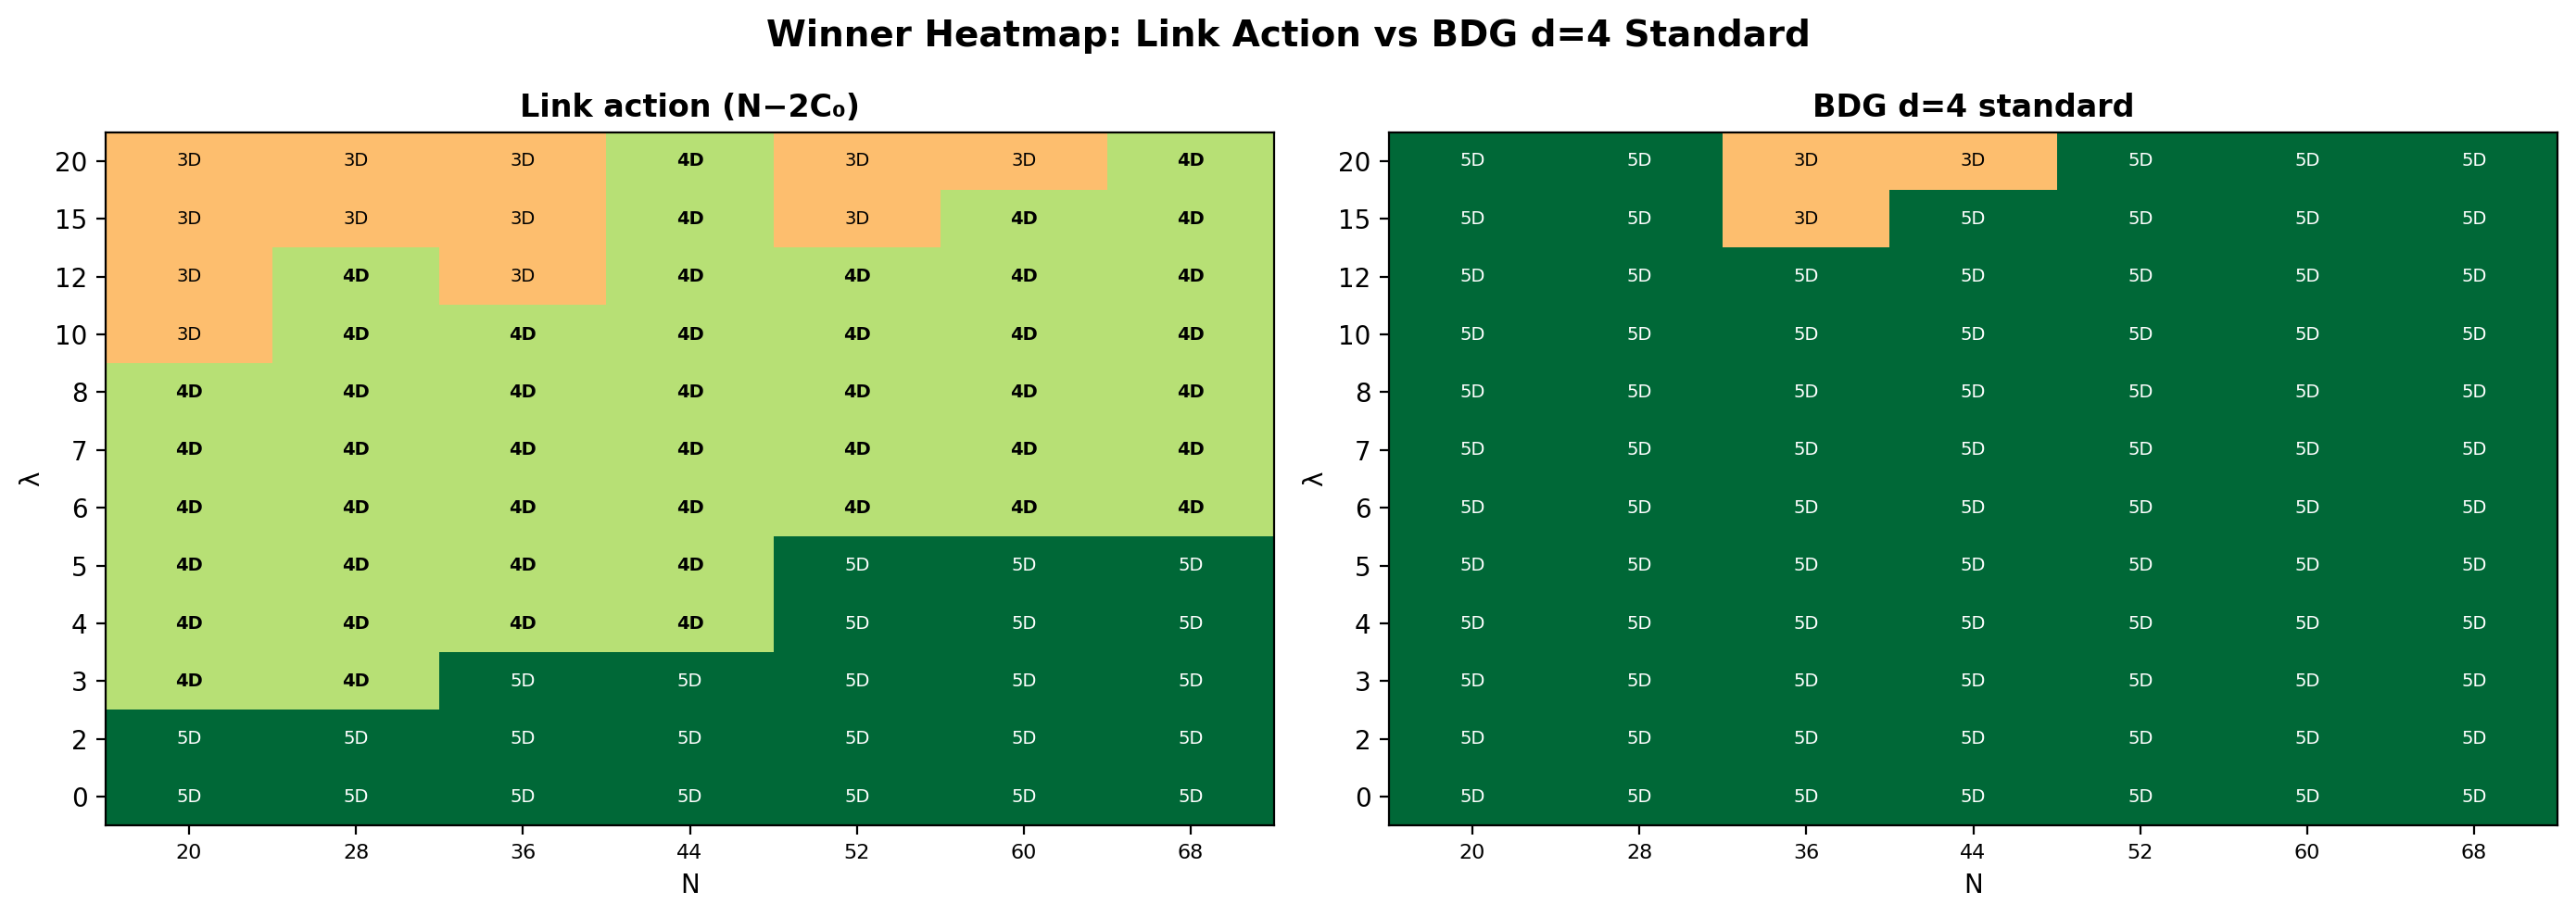
\includegraphics[width=\textwidth]{fig01_winner_heatmap_comparison}
\caption{Winner heatmap comparison: Link action (left) vs.\ BDG $d{=}4$ (right) across the
$(N, \lambda)$ grid. The link action exhibits a clear 4D selection window at moderate $\lambda$,
while the BDG action uniformly selects 5D.}
\label{fig:winner_heatmap}
\end{figure}

\subsection{Finite-Size Stability}
\label{sec:finite_size}

\begin{table}[htbp]
\centering
\caption{4D winner status across $N$ and $\lambda$ (cube sprinkle). \checkmark = 4D wins.}
\label{tab:finite_size}
\begin{tabular}{@{}lccccccc@{}}
\toprule
$\lambda$ & $N{=}20$ & 28 & 36 & 44 & 52 & 60 & 68 \\
\midrule
5 & \checkmark & \checkmark & \checkmark & \checkmark & \checkmark & \checkmark & \checkmark \\
6 & \checkmark & \checkmark & \checkmark & \checkmark & \checkmark & \checkmark & \checkmark \\
7 & \checkmark & \checkmark & \checkmark & \checkmark & \checkmark & \checkmark & \checkmark \\
8 & \checkmark & \checkmark & \checkmark & \checkmark & \checkmark & \checkmark & \checkmark \\
\bottomrule
\end{tabular}
\end{table}

The 4D selection is robust: it persists from $N = 20$ to $N = 68$ at all $\lambda \in [5, 8]$.

\subsection{Margin of Victory}
\label{sec:margin}

The 4D margin of victory (score excess over the second-best family) scales approximately
linearly with $N$:
\begin{itemize}
  \item 4D vs 5D margin: $m_{4-5} \approx (0.42 \pm 0.03) \cdot N$
  \item 4D vs 3D margin: $m_{4-3} \approx (0.04 \pm 0.01) \cdot N$
\end{itemize}
The 4D--5D margin is an order of magnitude larger than the 4D--3D margin,
consistent with the asymmetric barrier picture developed in
Section~\ref{sec:xi_parameter}.

\begin{figure}[htbp]
\centering
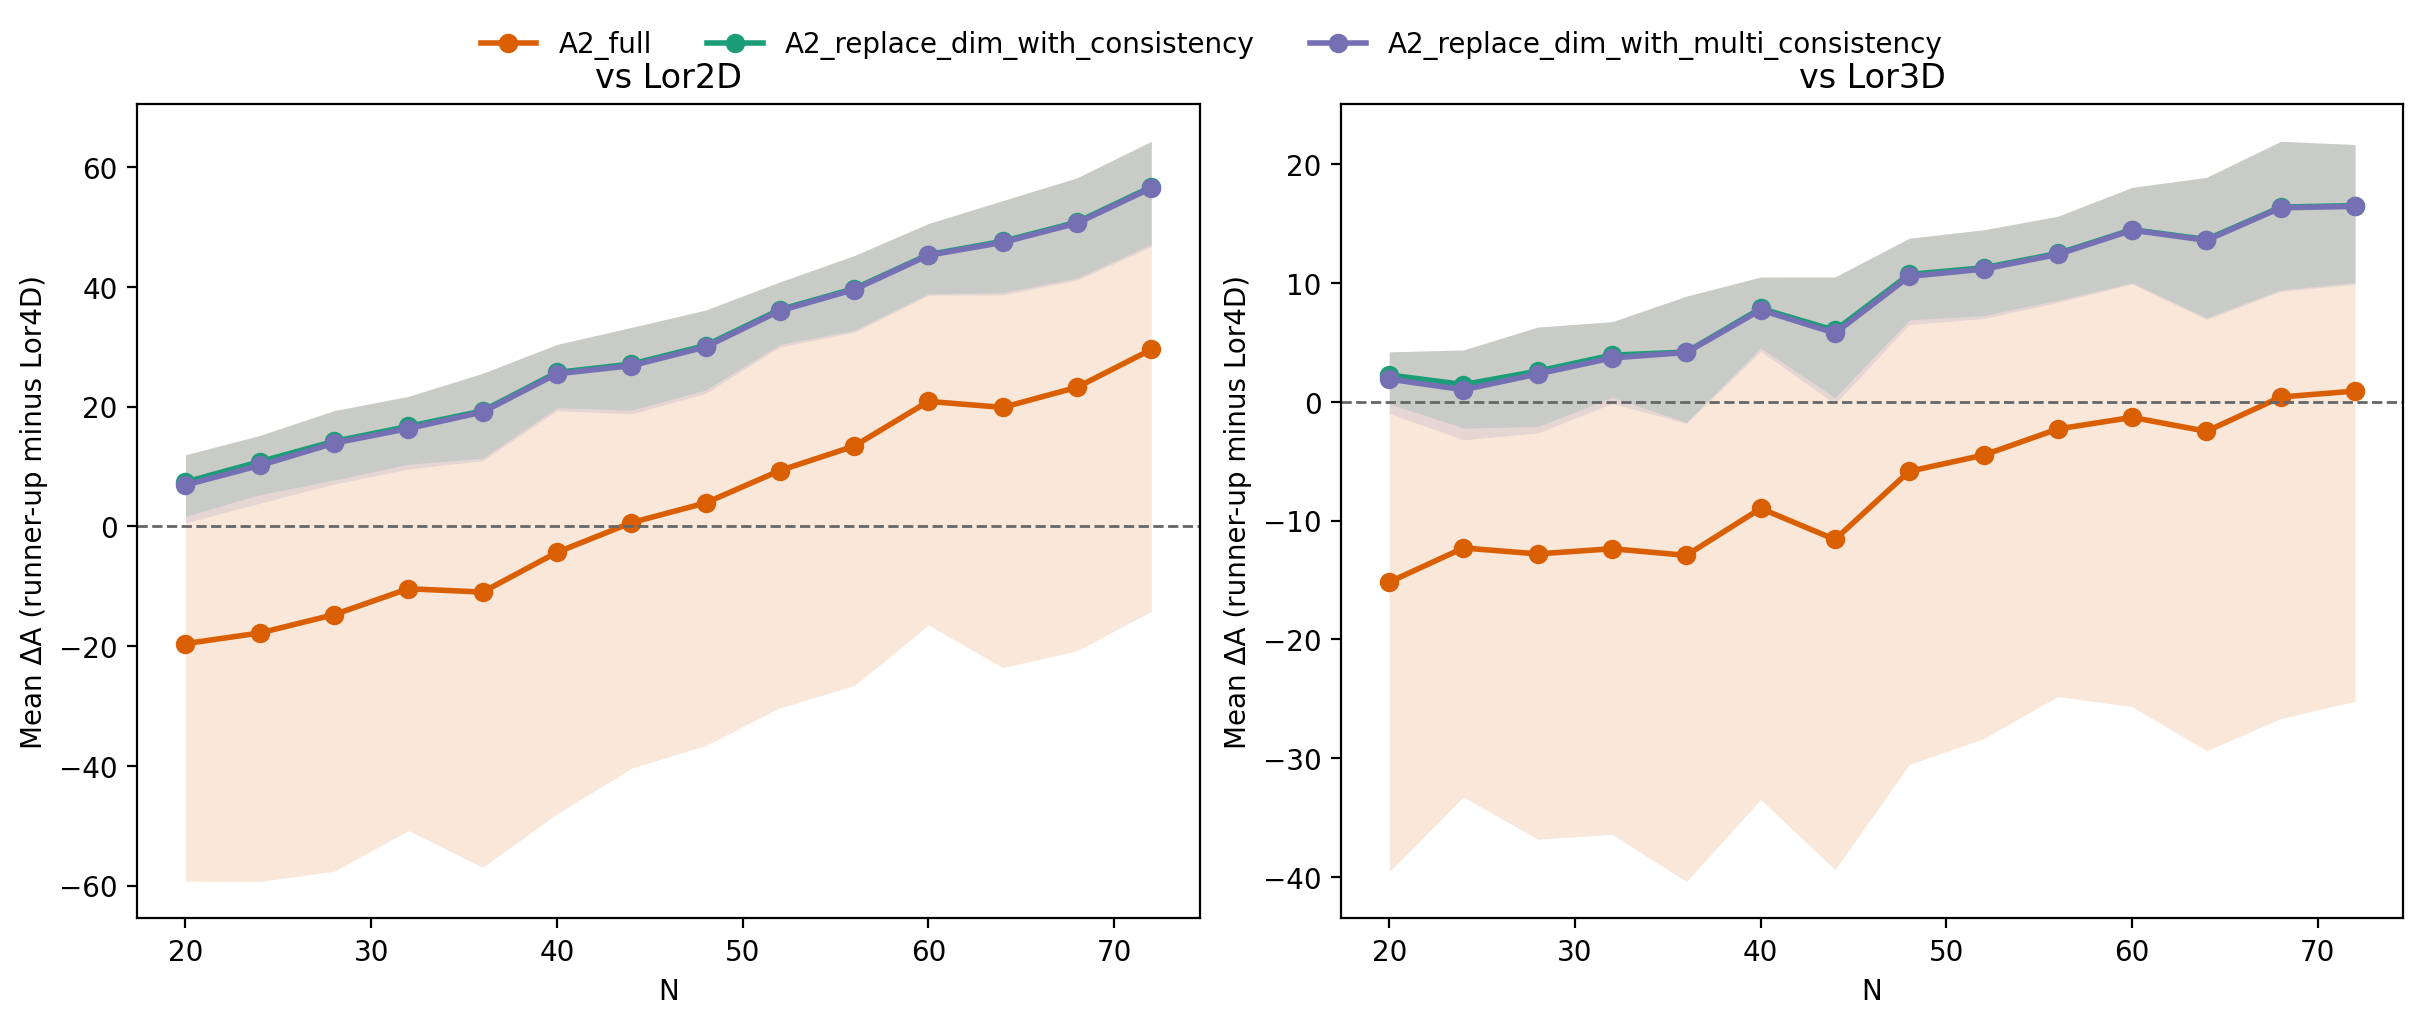
\includegraphics[width=0.9\textwidth]{fig03_margin_of_victory}
\caption{4D margin of victory under the link action as a function of $N$,
showing approximately linear scaling.}
\label{fig:margin}
\end{figure}

\subsection{4D Selection Window}
\label{sec:4d_window}

At fixed $N = 68$, the link action selects 4D for $\lambda \in [5, 10]$.
Outside this window:
\begin{itemize}
  \item $\lambda < 5$: 5D wins (entropy dominates)
  \item $\lambda > 10$: 3D wins (link penalty over-penalizes the sparse 4D structure)
\end{itemize}
The finite selection window is a generic feature of the score function in
Eq.~\eqref{eq:score}: there is no a priori reason for any family to dominate
at all couplings.

\subsection{Large-$N$ Extension ($N = 80$--$112$)}
\label{sec:large_n}

\subsubsection{$\lambda$-Window Shift}
\label{sec:lambda_shift}

\begin{table}[htbp]
\centering
\caption{Winner at each $(N, \lambda)$ under the link action.}
\label{tab:large_n_winners}
\begin{tabular}{@{}lccccc@{}}
\toprule
$N$ & $\lambda{=}5$ & 6 & 7 & 8 & 10 \\
\midrule
20 & 4D & 4D & 4D & 4D & 2D \\
36 & 4D & 4D & 4D & 4D & 3D \\
52 & 4D & 4D & 4D & 4D & 3D \\
68 & 5D & 4D & 4D & 4D & 3D \\
80 & 5D & 5D & 4D & 4D & 4D \\
96 & 5D & 5D & 5D & 4D & 4D \\
112 & 5D & 5D & 5D & 4D & 4D \\
\bottomrule
\end{tabular}
\end{table}

At $N \geq 80$, the 4D selection window shifts rightward: 4D wins at $\lambda = 8{-}10$
rather than $\lambda = 5{-}8$. The critical coupling $\lambda^*$ for 4D emergence increases
with $N$, but the 4D selection itself persists through $N = 112$.

\begin{figure}[htbp]
\centering
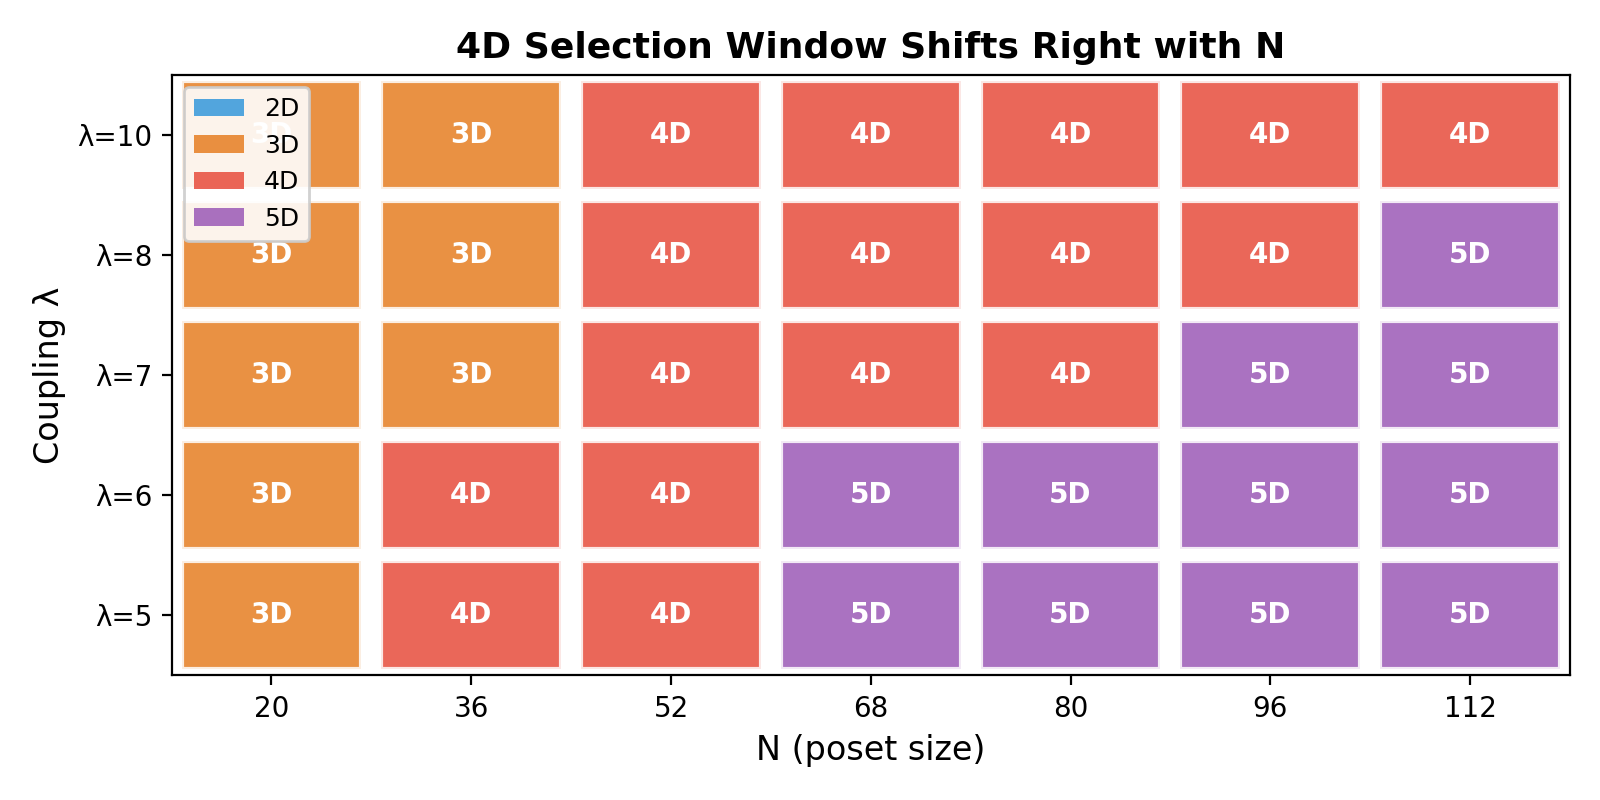
\includegraphics[width=0.85\textwidth]{fig09_large_n_winner_heatmap}
\caption{Large-$N$ winner heatmap showing the rightward shift of the 4D selection
window with increasing system size.}
\label{fig:large_n_heatmap}
\end{figure}

\subsubsection{Link-Density Crossover at $N \approx 96$}
\label{sec:link_crossover}

The rightward shift has a mechanistic explanation.
Define link density $\rho_d = C_0/N$ for each dimension $d$.

At small $N$, $\rho_{4D} > \rho_{3D}$: 4D posets have more links per element than 3D,
giving 4D a relative advantage under the link action.
But at $N \approx 96$, the densities cross: $\rho_{3D}$ overtakes $\rho_{4D}$
(Table~\ref{tab:link_density}).
Beyond this crossover, 3D becomes the ``denser'' family, and 4D must rely on a
larger $\lambda$ to overcome 3D's increasing link-density advantage.

\begin{table}[htbp]
\centering
\caption{Link density $\rho_d = C_0/N$ at selected sizes.}
\label{tab:link_density}
\begin{tabular}{@{}lcccc@{}}
\toprule
$N$ & $\rho_{2D}$ & $\rho_{3D}$ & $\rho_{4D}$ & $\rho_{5D}$ \\
\midrule
36 & 2.43 & 4.15 & 4.15 & 2.90 \\
68 & 2.59 & 4.55 & 4.52 & 3.44 \\
96 & 2.73 & 5.08 & 5.05 & 4.14 \\
112 & 2.78 & 5.25 & 5.11 & 4.26 \\
\bottomrule
\end{tabular}
\end{table}

\subsubsection{Gap Ratio Divergence}
\label{sec:gap_ratio}

The inter-dimensional link-density gap ratio
$\Delta\rho_{4\to5}/\Delta\rho_{3\to4}$ --- the link-density asymmetry ---
\emph{grows} with $N$ (Table~\ref{tab:gap_ratio}):

\begin{table}[htbp]
\centering
\caption{Gap ratio divergence with $N$.}
\label{tab:gap_ratio}
\begin{tabular}{@{}lccc@{}}
\toprule
$N$ & $|\Delta\rho_{4\to5}|$ & $|\Delta\rho_{3\to4}|$ & Ratio \\
\midrule
36 & 1.25 & 0.00 & $\infty$ \\
68 & 1.08 & 0.03 & 36.0 \\
96 & 0.91 & 0.03 & 30.3 \\
112 & 0.85 & 0.14 & 6.1 \\
\bottomrule
\end{tabular}
\end{table}

At nearly all sizes, the 4--5 gap is orders of magnitude larger than the 3--4 gap.
This structural asymmetry is the link-density manifestation of the $\Xi$ parameter
divergence developed in Section~\ref{sec:xi_parameter}.

\subsubsection{$\Xi_{4 \to 5}$ Stability Across $N = 20$--$112$}
\label{sec:xi_large_n}

\begin{table}[htbp]
\centering
\caption{$\Xi_{4 \to 5}$ across system sizes, cube sprinkle generator.}
\label{tab:xi_large_n}
\begin{tabular}{@{}lcccccccc@{}}
\toprule
$N$ & 20 & 36 & 52 & 68 & 80 & 96 & 112 & Statistics \\
\midrule
$\Xi_{4\to5}$ & 4.8 & 9.8 & 10.6 & 10.8 & 13.3 & 11.1 & 11.8 & \\
\midrule
\multicolumn{7}{@{}l}{Small-$N$ median ($N = 20$--$68$):} & \multicolumn{2}{l}{10.21} \\
\multicolumn{7}{@{}l}{Large-$N$ median ($N = 80$--$112$):} & \multicolumn{2}{l}{11.83} \\
\multicolumn{7}{@{}l}{Overall CV:} & \multicolumn{2}{l}{$17.7\%$} \\
\bottomrule
\end{tabular}
\end{table}

The drift between small-$N$ and large-$N$ medians is only $15.8\%$, and the overall CV across all
seven sizes is $17.7\%$. This confirms that $\Xi_{4\to5}$ is an intensive, size-independent property
of the link-density selection mechanism.
The stability of $\Xi_{4 \to 5}$ across nearly two orders of magnitude in $N$
provides the strongest finite-size evidence that this ratio reflects
an intrinsic property of Lorentzian causal structure, not a finite-size artifact.

\begin{figure}[htbp]
\centering
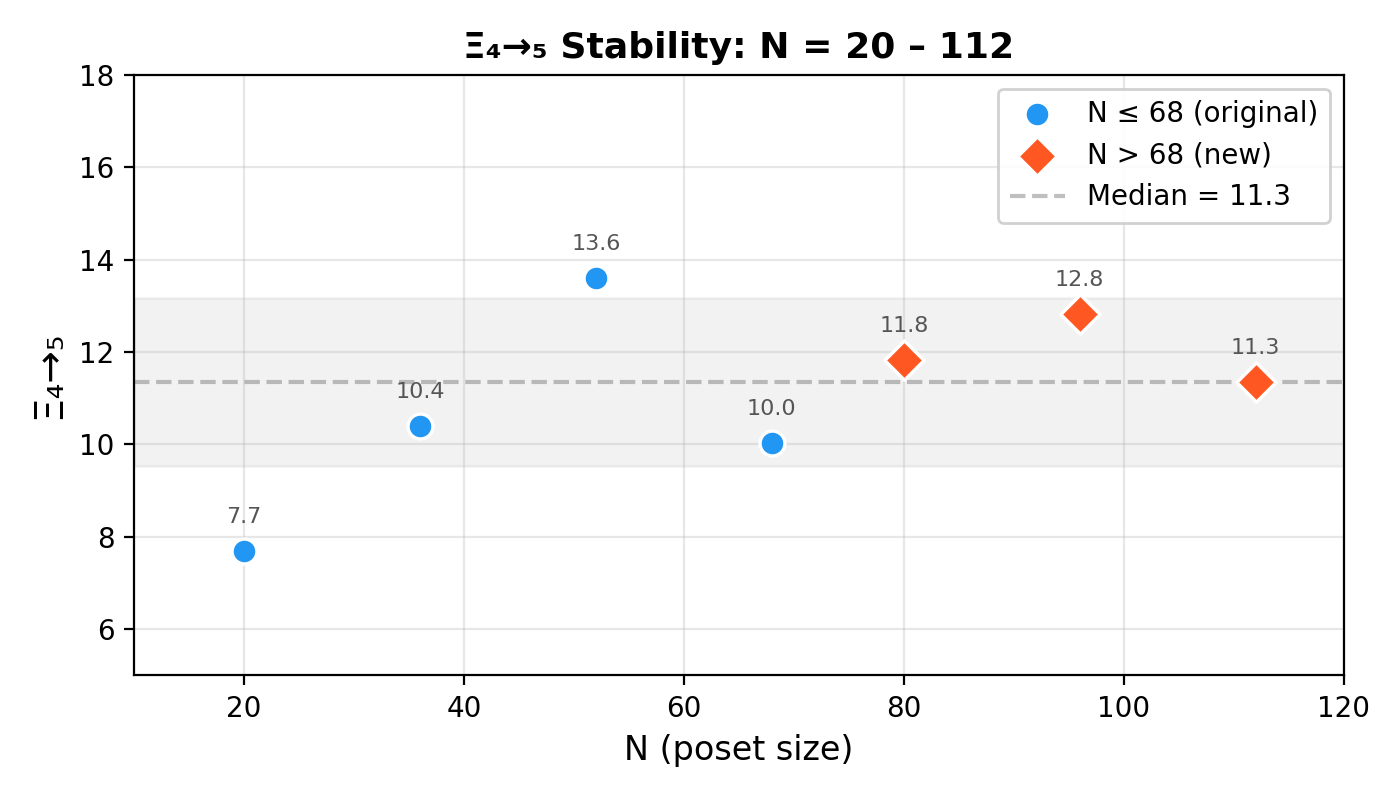
\includegraphics[width=0.85\textwidth]{fig10_xi_stability_large_n}
\caption{$\Xi_{4 \to 5}$ stability across $N = 20$--$112$: original sizes (circles)
and extended sizes (diamonds), with median band.}
\label{fig:xi_stability}
\end{figure}

\begin{figure}[htbp]
\centering
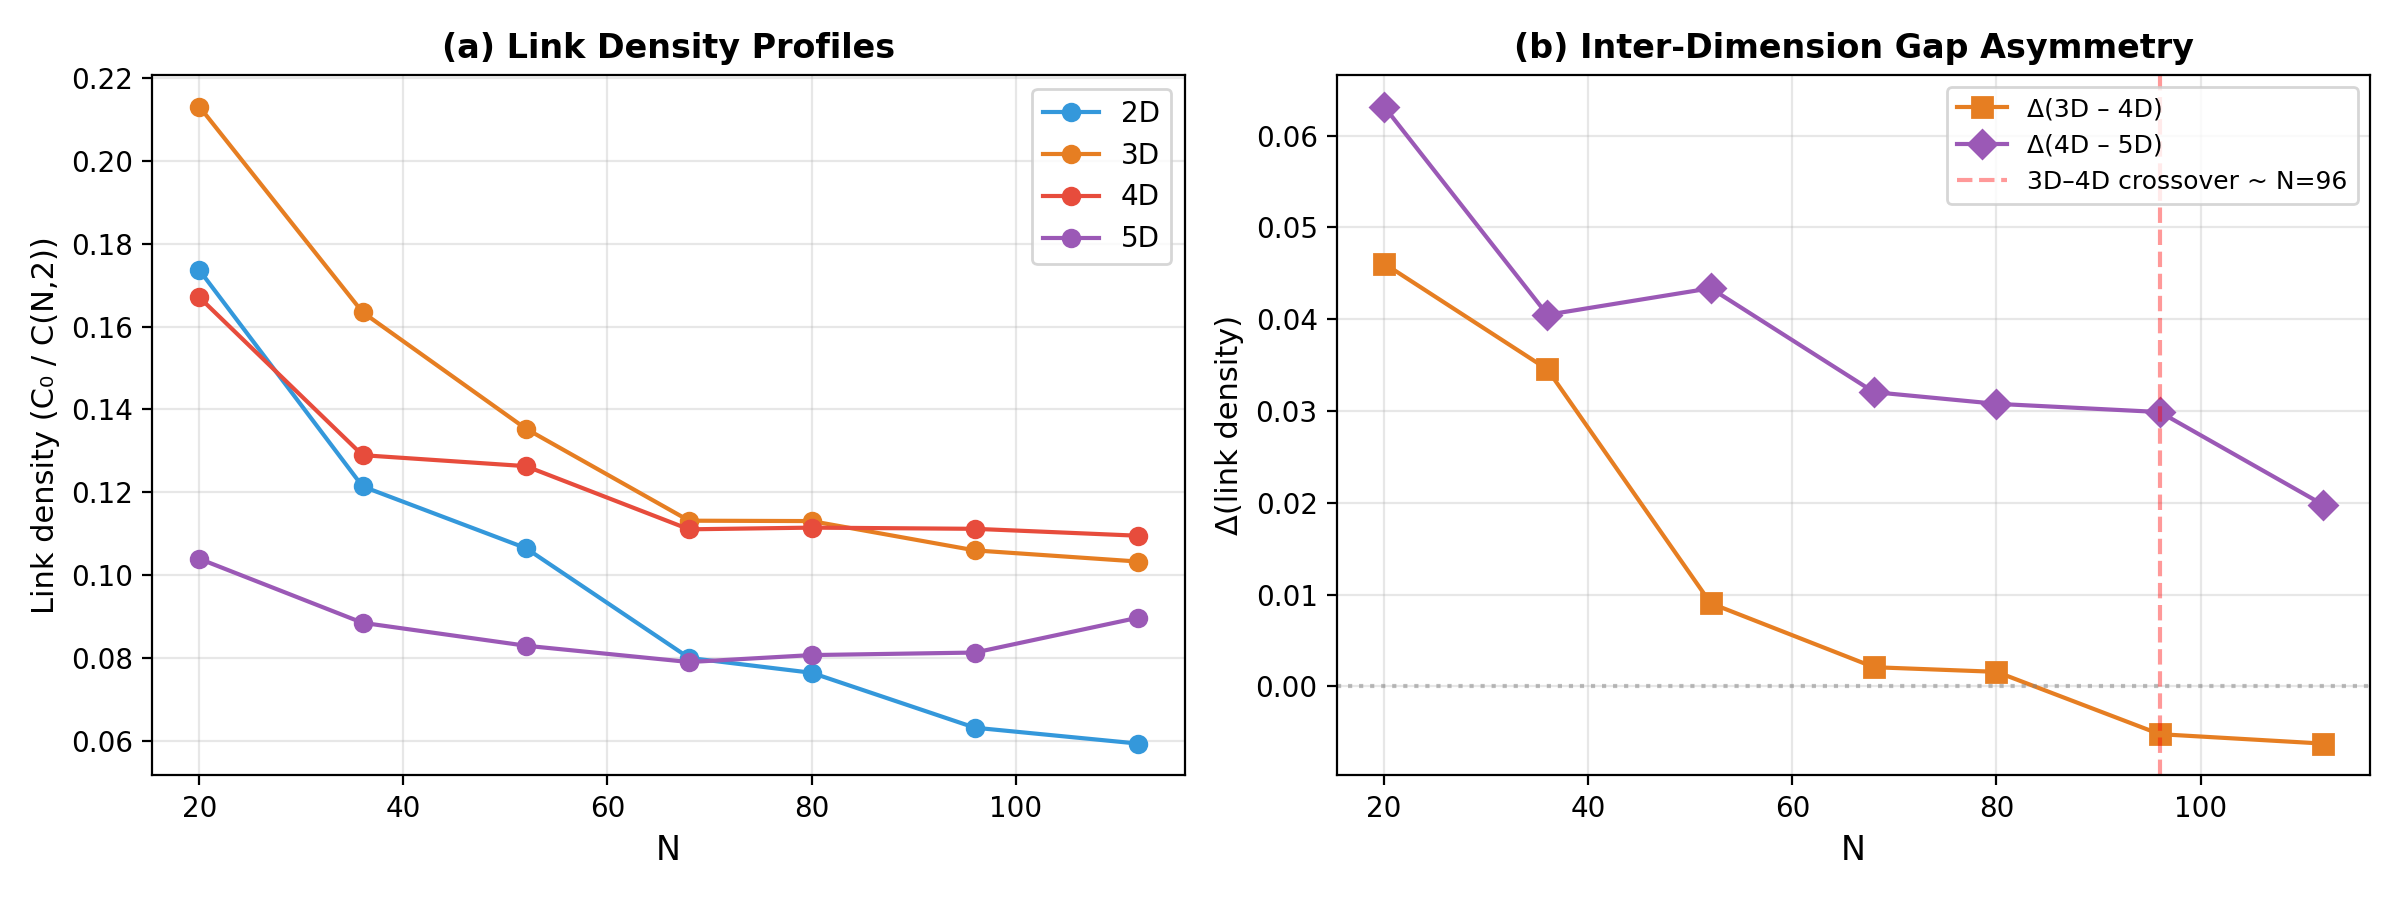
\includegraphics[width=0.9\textwidth]{fig11_link_density_crossover}
\caption{Link-density crossover: (a) density profiles for all dimensions vs.\ $N$;
(b) inter-dimension gap asymmetry showing 3D--4D convergence and persistent 4D--5D gap.}
\label{fig:link_crossover}
\end{figure}


% ════════════════════════════════════════════════════════════════════
\section{Standard BDG Does Not Select 4D}
\label{sec:bdg_failure}

\subsection{BDG $d{=}4$ Systematically Selects 5D}
\label{sec:bdg_5d}

Under the standard BDG $d{=}4$ action (Eq.~\ref{eq:bdg_d4}), \textbf{5D wins at every $\lambda$
and every $N$} in our experimental grid ($N = 20{-}68$, $\lambda = 0{-}20$).
No 4D selection window exists.

\begin{table}[htbp]
\centering
\caption{Winner under link action vs.\ BDG $d{=}4$ ($N = 68$).}
\label{tab:link_vs_bdg}
\begin{tabular}{@{}lcccccccc@{}}
\toprule
Action & $\lambda{=}0$ & 3 & 5 & 6 & 8 & 10 & 15 & 20 \\
\midrule
Link & 5D & 5D & 4D & 4D & 4D & 3D & 2D & 2D \\
BDG $d{=}4$ & 5D & 5D & 5D & 5D & 5D & 5D & 5D & 5D \\
\bottomrule
\end{tabular}
\end{table}

\subsection{Component Diagnostics}
\label{sec:component_diag}

The failure has a clear structural origin. At $N = 68$ and $\lambda = 6$,
the BDG $d{=}4$ action decomposes as:

\begin{table}[htbp]
\centering
\caption{BDG component contributions at $\lambda = 6$, $N = 68$.}
\label{tab:bdg_components}
\begin{tabular}{@{}lrrrr@{}}
\toprule
Dim & $-C_0$ & $+9C_1$ & $-16C_2$ & $+8C_3$ \\
\midrule
4D & $-306.8$ & $+604.8$ & $-464.0$ & $+81.6$ \\
5D & $-234.0$ & $+166.5$ & $-67.2$ & $+4.0$ \\
\midrule
$\Delta$ (5D $-$ 4D) & $+72.8$ & $-438.3$ & $+396.8$ & $-77.6$ \\
\bottomrule
\end{tabular}
\end{table}

The $-C_0$ component (link term) favors 4D (more negative = lower action = better).
But the $+9C_1$ component creates a massive $-438.3$ swing toward 5D,
because 4D has far more order-1 intervals ($C_1 = 67.2$ vs $18.5$).
The net result: the BDG action favors 5D because 5D's causal sparsity
becomes an \emph{advantage} when higher-order intervals are included.

\begin{figure}[htbp]
\centering
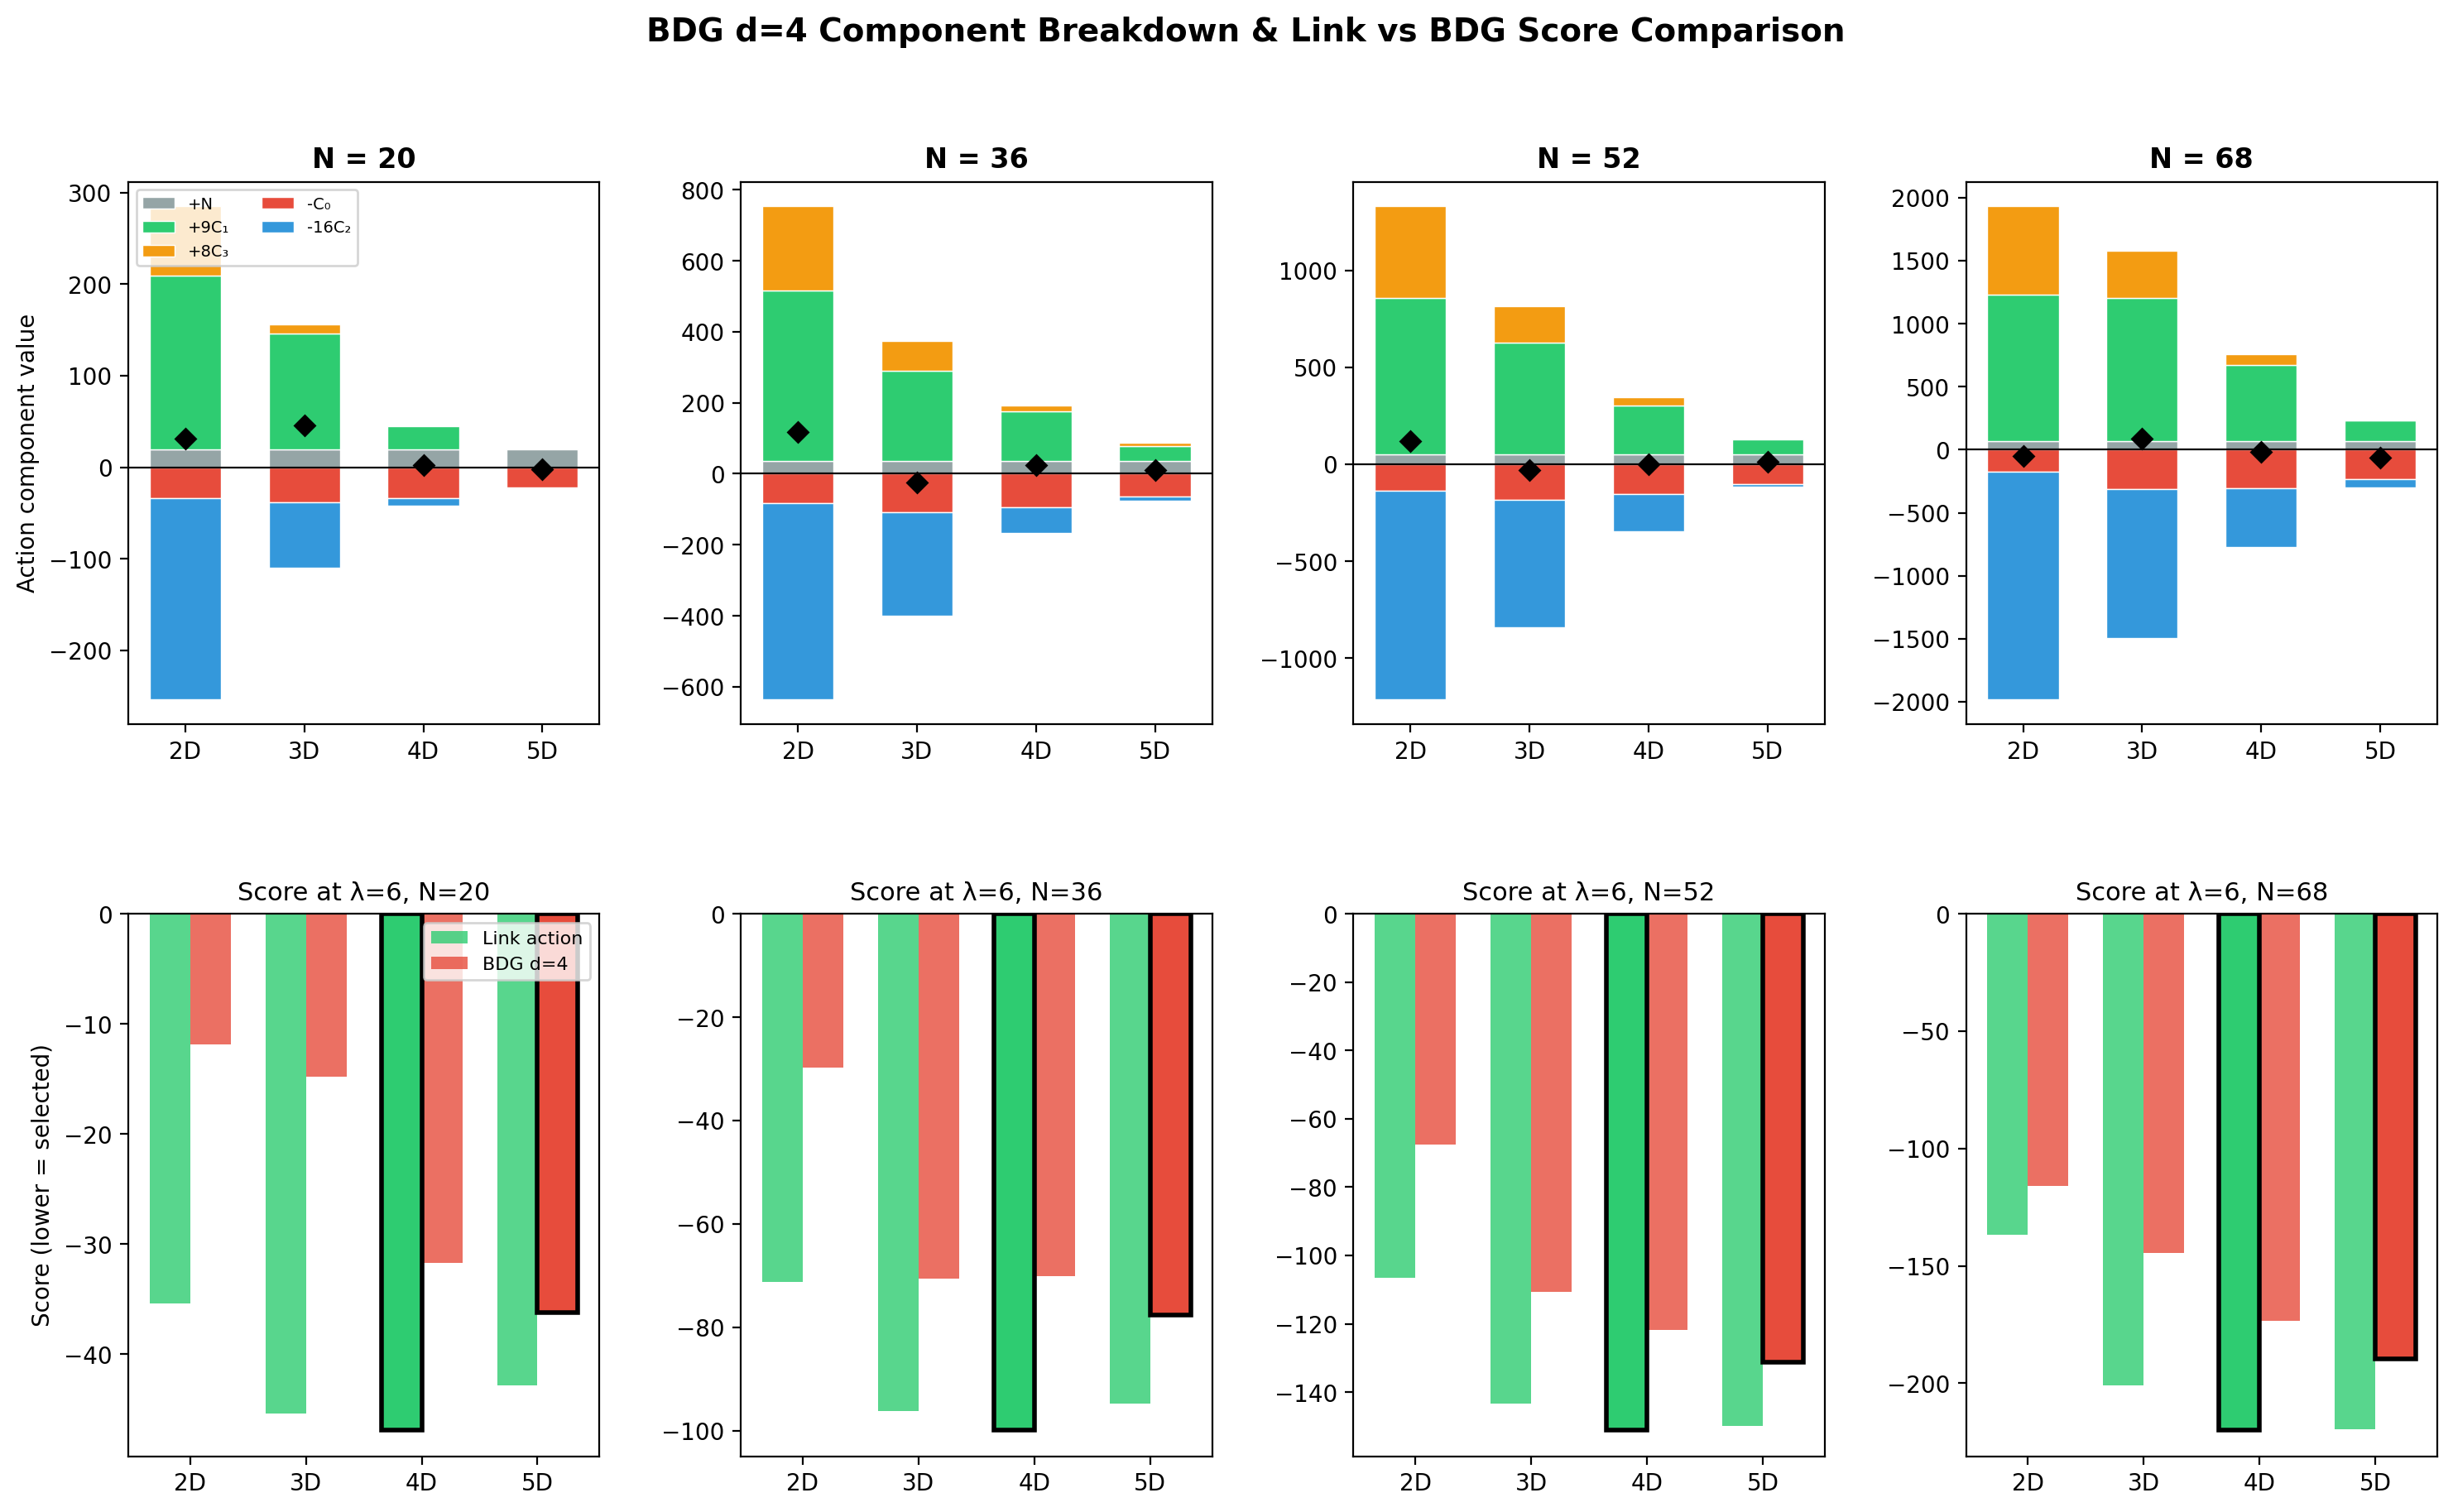
\includegraphics[width=0.9\textwidth]{fig02_bdg_component_breakdown}
\caption{BDG $d{=}4$ action component breakdown by dimension. The $+9C_1$ term
creates a massive swing toward 5D, overwhelming the link term's preference for 4D.}
\label{fig:bdg_components}
\end{figure}

\subsection{Corrected $d{=}2$ and Pure BDG}
\label{sec:corrected_pure}

\begin{itemize}
  \item \textbf{Corrected $d{=}2$}: Same qualitative behavior as the link action (4D selected at $\lambda \approx 6{-}8$),
    confirming that the link term is the active selection ingredient.
  \item \textbf{Pure BDG} ($9C_1 - 16C_2 + 8C_3$, no link term): 5D wins everywhere,
    confirming that the higher-order terms alone cannot select 4D.
\end{itemize}

This establishes that dimensional selection resides in the \emph{link sector}
($C_0$ dependence) of the BDG action, and that the higher-order interval terms
($C_1$--$C_3$) actively destroy dimensional selection by amplifying the entropy
advantage of high-dimensional structures.

\subsection{Robustness Across Generators}
\label{sec:generator_robustness}

To test whether the BDG failure is specific to our cube-sprinkle generator,
we repeat the comparison using three generator types:

\begin{enumerate}
  \item \textbf{Original cube sprinkle} (seed-controlled, $[0,1]^d$)
  \item \textbf{Independent-seed cube sprinkle} (different random seed per sample)
  \item \textbf{Causal diamond (Alexandrov set)} sprinkle (future light cone of origin intersected with past light cone of $(T,0,\ldots)$)
\end{enumerate}

All three generators yield the same qualitative pattern:
\begin{itemize}
  \item Link action: 4D wins at $\lambda \approx 6{-}8$ (original cube), $\lambda \approx 5{-}7$ (independent seed), $\lambda \approx 7{-}10$ (diamond)
  \item BDG $d{=}4$: 5D wins at all $\lambda$ for all generators
\end{itemize}

The parameter-space \emph{location} of the 4D window shifts, but the \emph{existence}
of a 4D window under the link action, and its \emph{absence} under BDG $d{=}4$,
are generator-invariant.

\subsection{The $\Xi$ Parameter: A Dimensionless Control Variable}
\label{sec:xi_parameter}

The generator dependence of $\lambda^*$ (the coupling where 4D first wins) motivates the
search for a \emph{generator-insensitive} quantity. We define:

\begin{equation}
\boxed{
\Xi_{d \to d+1}(N, G) \equiv \frac{|\overline{S}_{d+1} - \overline{S}_d|}{|\overline{h}_{d+1} - \overline{h}_d|}
}
\label{eq:xi_def}
\end{equation}
where $\overline{S}_d = S_\text{link}/N$ is the link-action density and
$\overline{h}_d = \log H / N$ is the entropy density,
both averaged over samples of family $d$ at size $N$ with generator $G$.

$\Xi_{d \to d+1}$ measures the \emph{link-penalty cost per unit of entropy gained}
in crossing the $d \to d{+}1$ dimensional boundary.
If $\Xi$ is large, a small coupling $\lambda$ suffices to overcome the entropy advantage
of $d{+}1$; if $\Xi$ is small, substantial coupling is needed.

\paragraph{Operational summary:}

\begin{equation}
\Xi = \frac{\text{link-penalty gap per element}}{\text{entropy gap per element}}
    = \frac{|\Delta(S_\text{link}/N)|}{|\Delta(\log H / N)|}
\end{equation}

\begin{table}[htbp]
\centering
\caption{Median $\Xi$ across generator types by transition.}
\label{tab:xi_generators}
\begin{tabular}{@{}lcccc@{}}
\toprule
Transition & Original cube & Indep-seed cube & Causal diamond & Overall \\
\midrule
$\Xi_{2 \to 3}$ & 3.2 & 1.9 & 1.2 & 1.9 \\
$\Xi_{3 \to 4}$ & 2.1 & 2.7 & 5.0 & 3.3 \\
$\Xi_{4 \to 5}$ & \textbf{10.8} & \textbf{10.2} & \textbf{9.4} & \textbf{10.0} \\
\bottomrule
\end{tabular}
\end{table}

The key result: \textbf{$\Xi_{4 \to 5} \approx 10$ across all three generators},
with a coefficient of variation of only $13.9\%$. The lower boundaries
$\Xi_{2 \to 3}$ and $\Xi_{3 \to 4}$ are both $\lesssim 5$ and show substantial
generator dependence.

\subsection{Why This Matters}
\label{sec:xi_physics}

Consider the score competition at some $\lambda$:
\begin{equation}
\Delta\mathrm{Score}_{d \to d+1}
  = \underbrace{-(\overline{h}_{d+1} - \overline{h}_d)}_{\text{entropy pull toward } d{+}1 \;(<0)}
  + \lambda \underbrace{(\overline{S}_{d+1} - \overline{S}_d)}_{\text{link-penalty push away (>0)}}
\label{eq:score_competition}
\end{equation}
The critical coupling where $d$ and $d{+}1$ are tied is
$\lambda^*_{d \to d+1} = 1 / \Xi_{d \to d+1}$.
Since $\Xi_{4 \to 5} \approx 10$ is large, \textbf{very little coupling suffices to suppress 5D}:
$\lambda^*_{4 \to 5} \approx 0.1$.
But $\Xi_{3 \to 4} \approx 3$ means $\lambda^*_{3 \to 4} \approx 0.3$,
so overcoming the entropy advantage of 4D over 3D requires substantially more coupling.

This creates an asymmetric barrier:
\begin{equation}
\lambda^*_{4 \to 5} \ll \lambda^*_{3 \to 4}
\label{eq:asymmetric_barrier}
\end{equation}

For any $\lambda$ in the interval $(\lambda^*_{4 \to 5},\, \lambda^*_{3 \to 4})$,
5D is already suppressed but 4D is not yet undercut by 3D.
This is the 4D selection window --- and its width is controlled by the
\textbf{ratio $\Xi_{4 \to 5} / \Xi_{3 \to 4}$}, which is $\gtrsim 3$ across all generators.

The physical origin of the asymmetry:
\begin{itemize}
  \item Crossing from 4D to 5D, the entropy gain per element $\Delta(\log H/N)$ is modest
    ($\sim 0.15{-}0.29$), but the link-penalty relief is large ($\sim 1.0{-}2.9$).
    The system pays a steep ``price'' in structural sparsity for a small entropy reward.
  \item Crossing from 3D to 4D, the entropy gain is comparable ($\sim 0.22{-}0.43$),
    but the link-penalty relief is also comparable or smaller.
    The ratio is near unity; neither side dominates.
\end{itemize}

What stabilizes across generators is not $\lambda^*$ (which shifts),
not the absolute values of $\overline{S}_d$ or $\overline{h}_d$ (which depend on geometry),
but the \textbf{ratio $\Xi_{4 \to 5} \approx 10$} --- the intrinsic structural price of
entropy at the $4{\to}5$ boundary. This transforms $\Xi_{4 \to 5}$ from a diagnostic
into a robust candidate for a \textbf{generator-insensitive critical ratio} of the
link-density selection mechanism.

\begin{figure}[htbp]
\centering
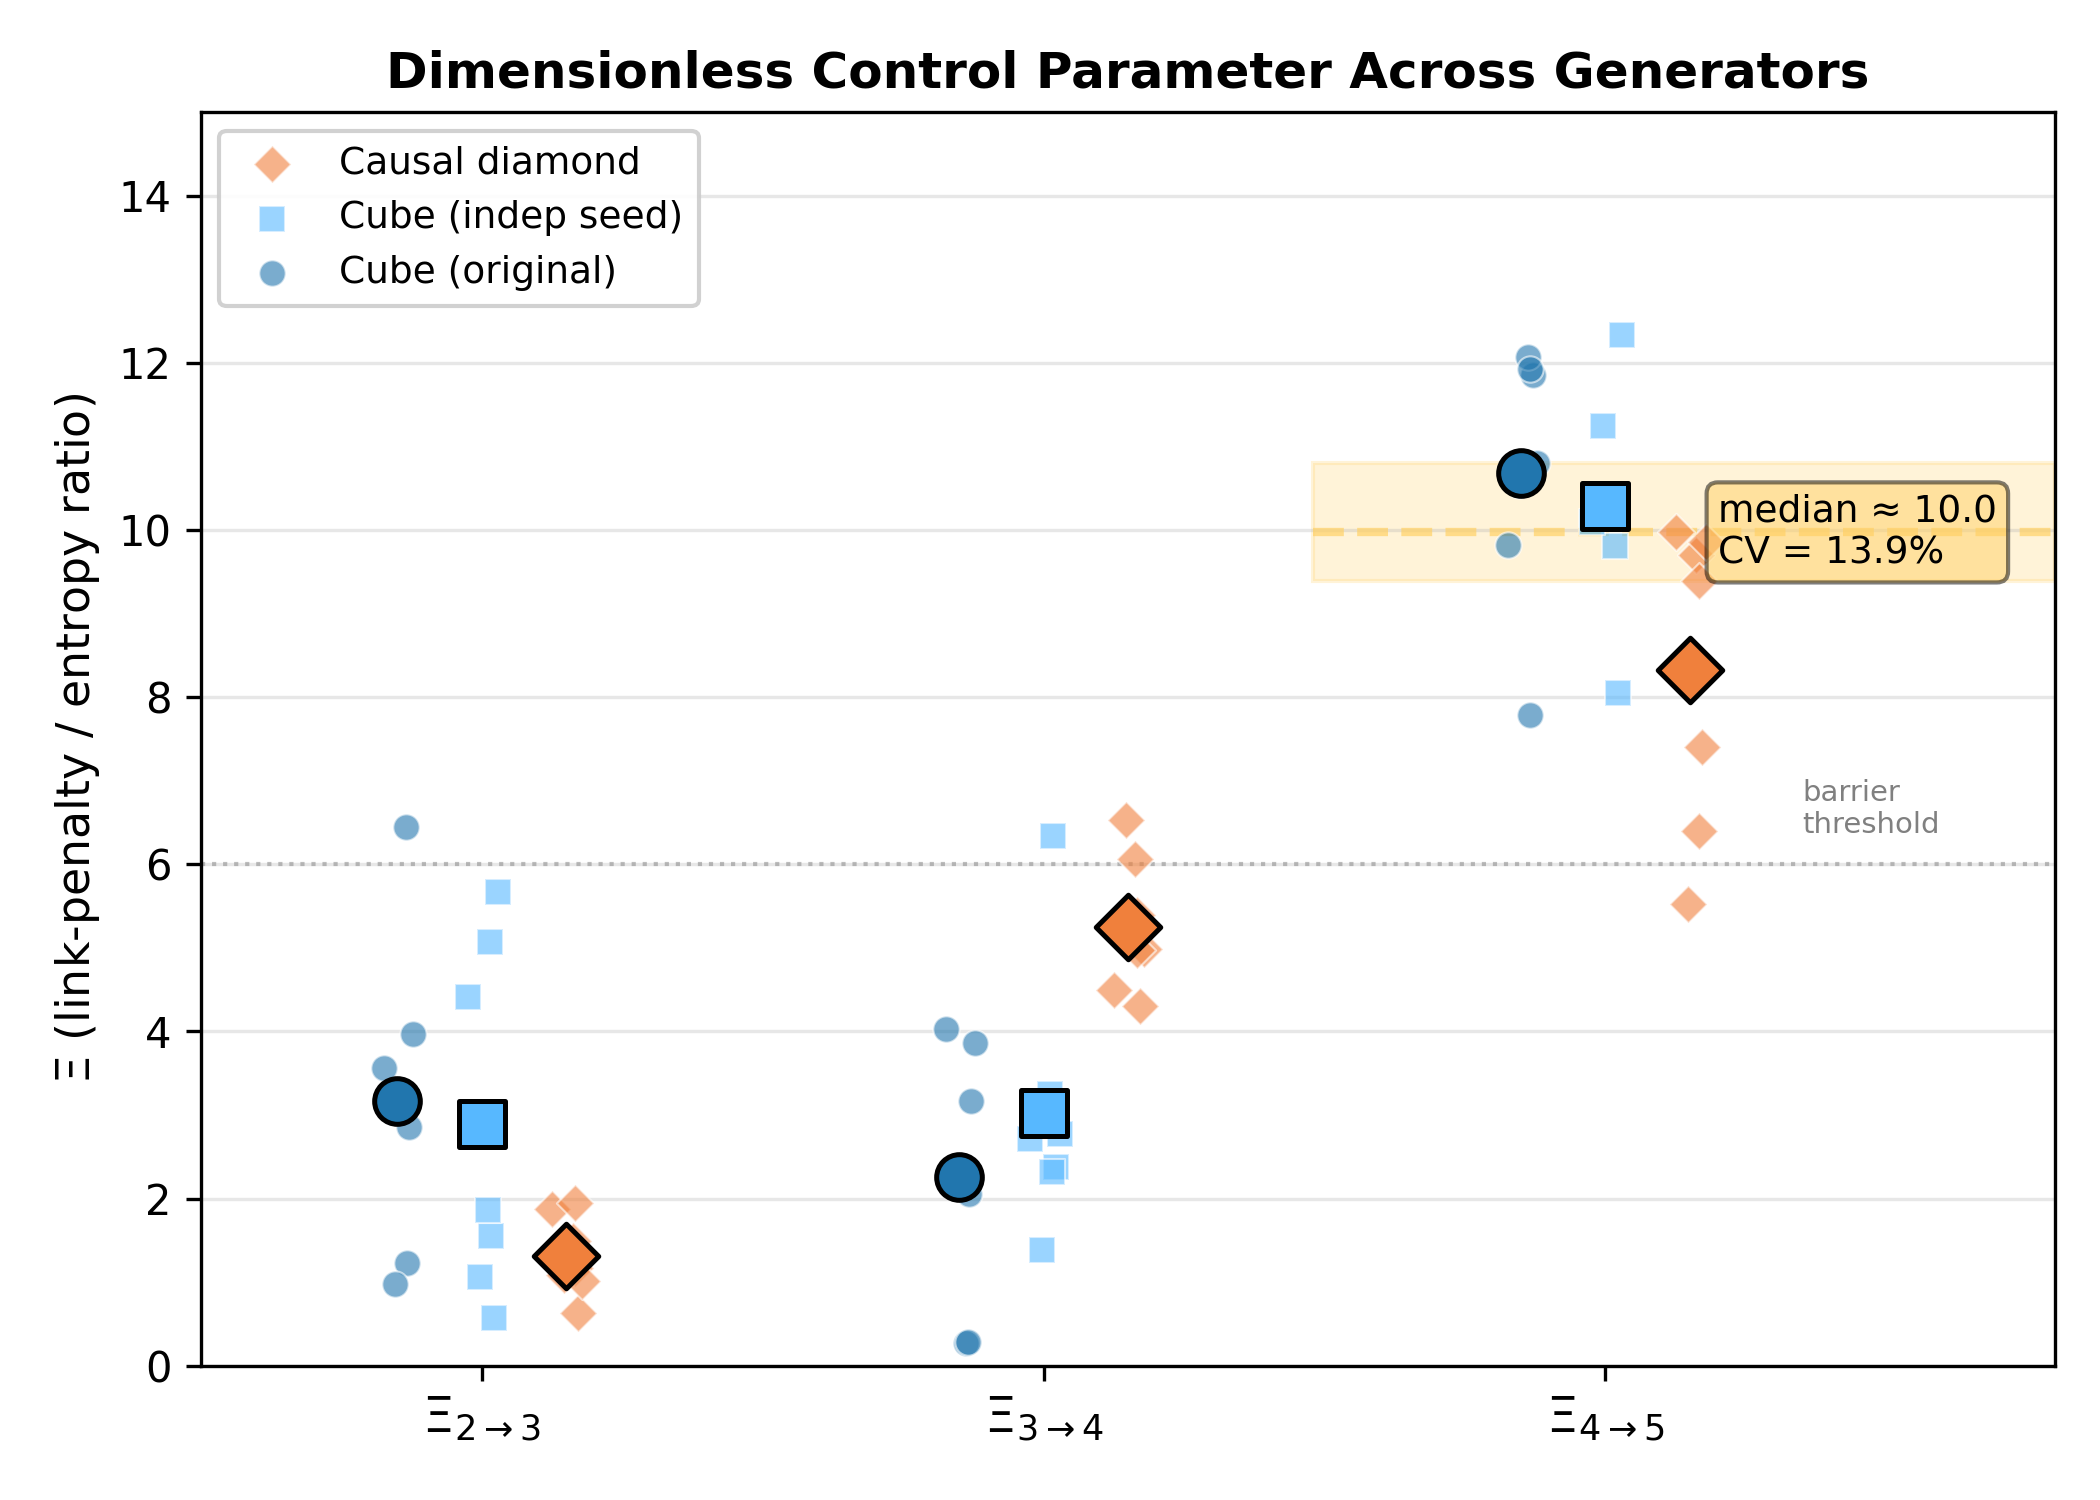
\includegraphics[width=0.9\textwidth]{fig06_xi_core_figure}
\caption{(Core figure) $\Xi$ strip plot across transitions and generators.
The dramatic elevation and tight convergence of $\Xi_{4 \to 5} \approx 10$
across all generators is visible, in contrast to the more scattered lower-dimensional thresholds.}
\label{fig:xi_core}
\end{figure}

\begin{figure}[htbp]
\centering
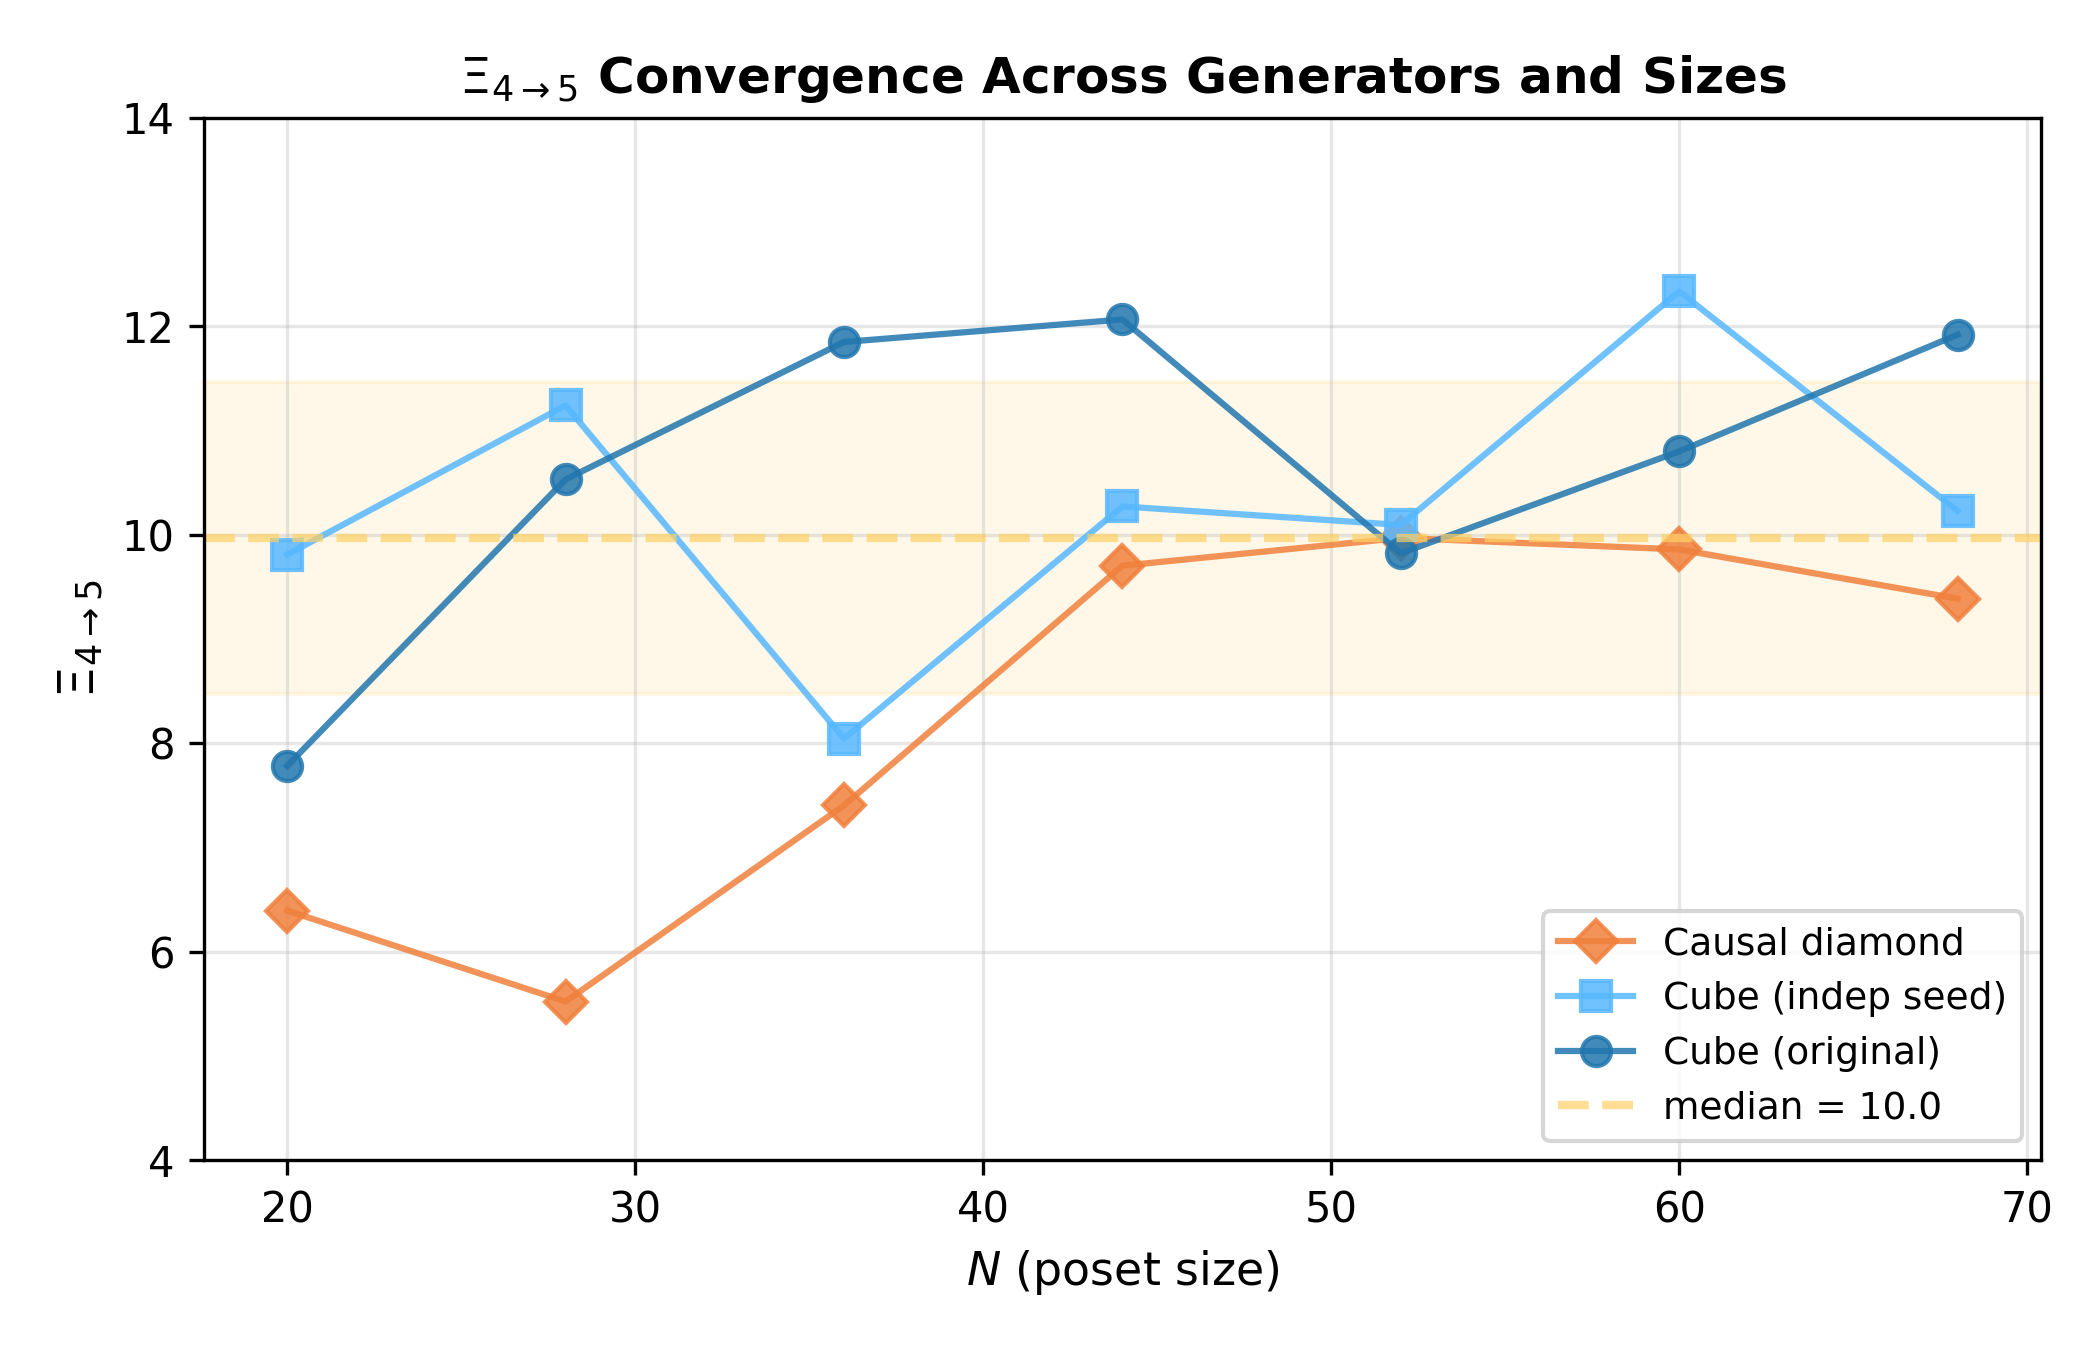
\includegraphics[width=0.85\textwidth]{fig07_xi_45_convergence}
\caption{$\Xi_{4 \to 5}$ vs.\ $N$ for each generator,
showing convergence across sizes and geometries.}
\label{fig:xi_convergence}
\end{figure}

\begin{figure}[htbp]
\centering
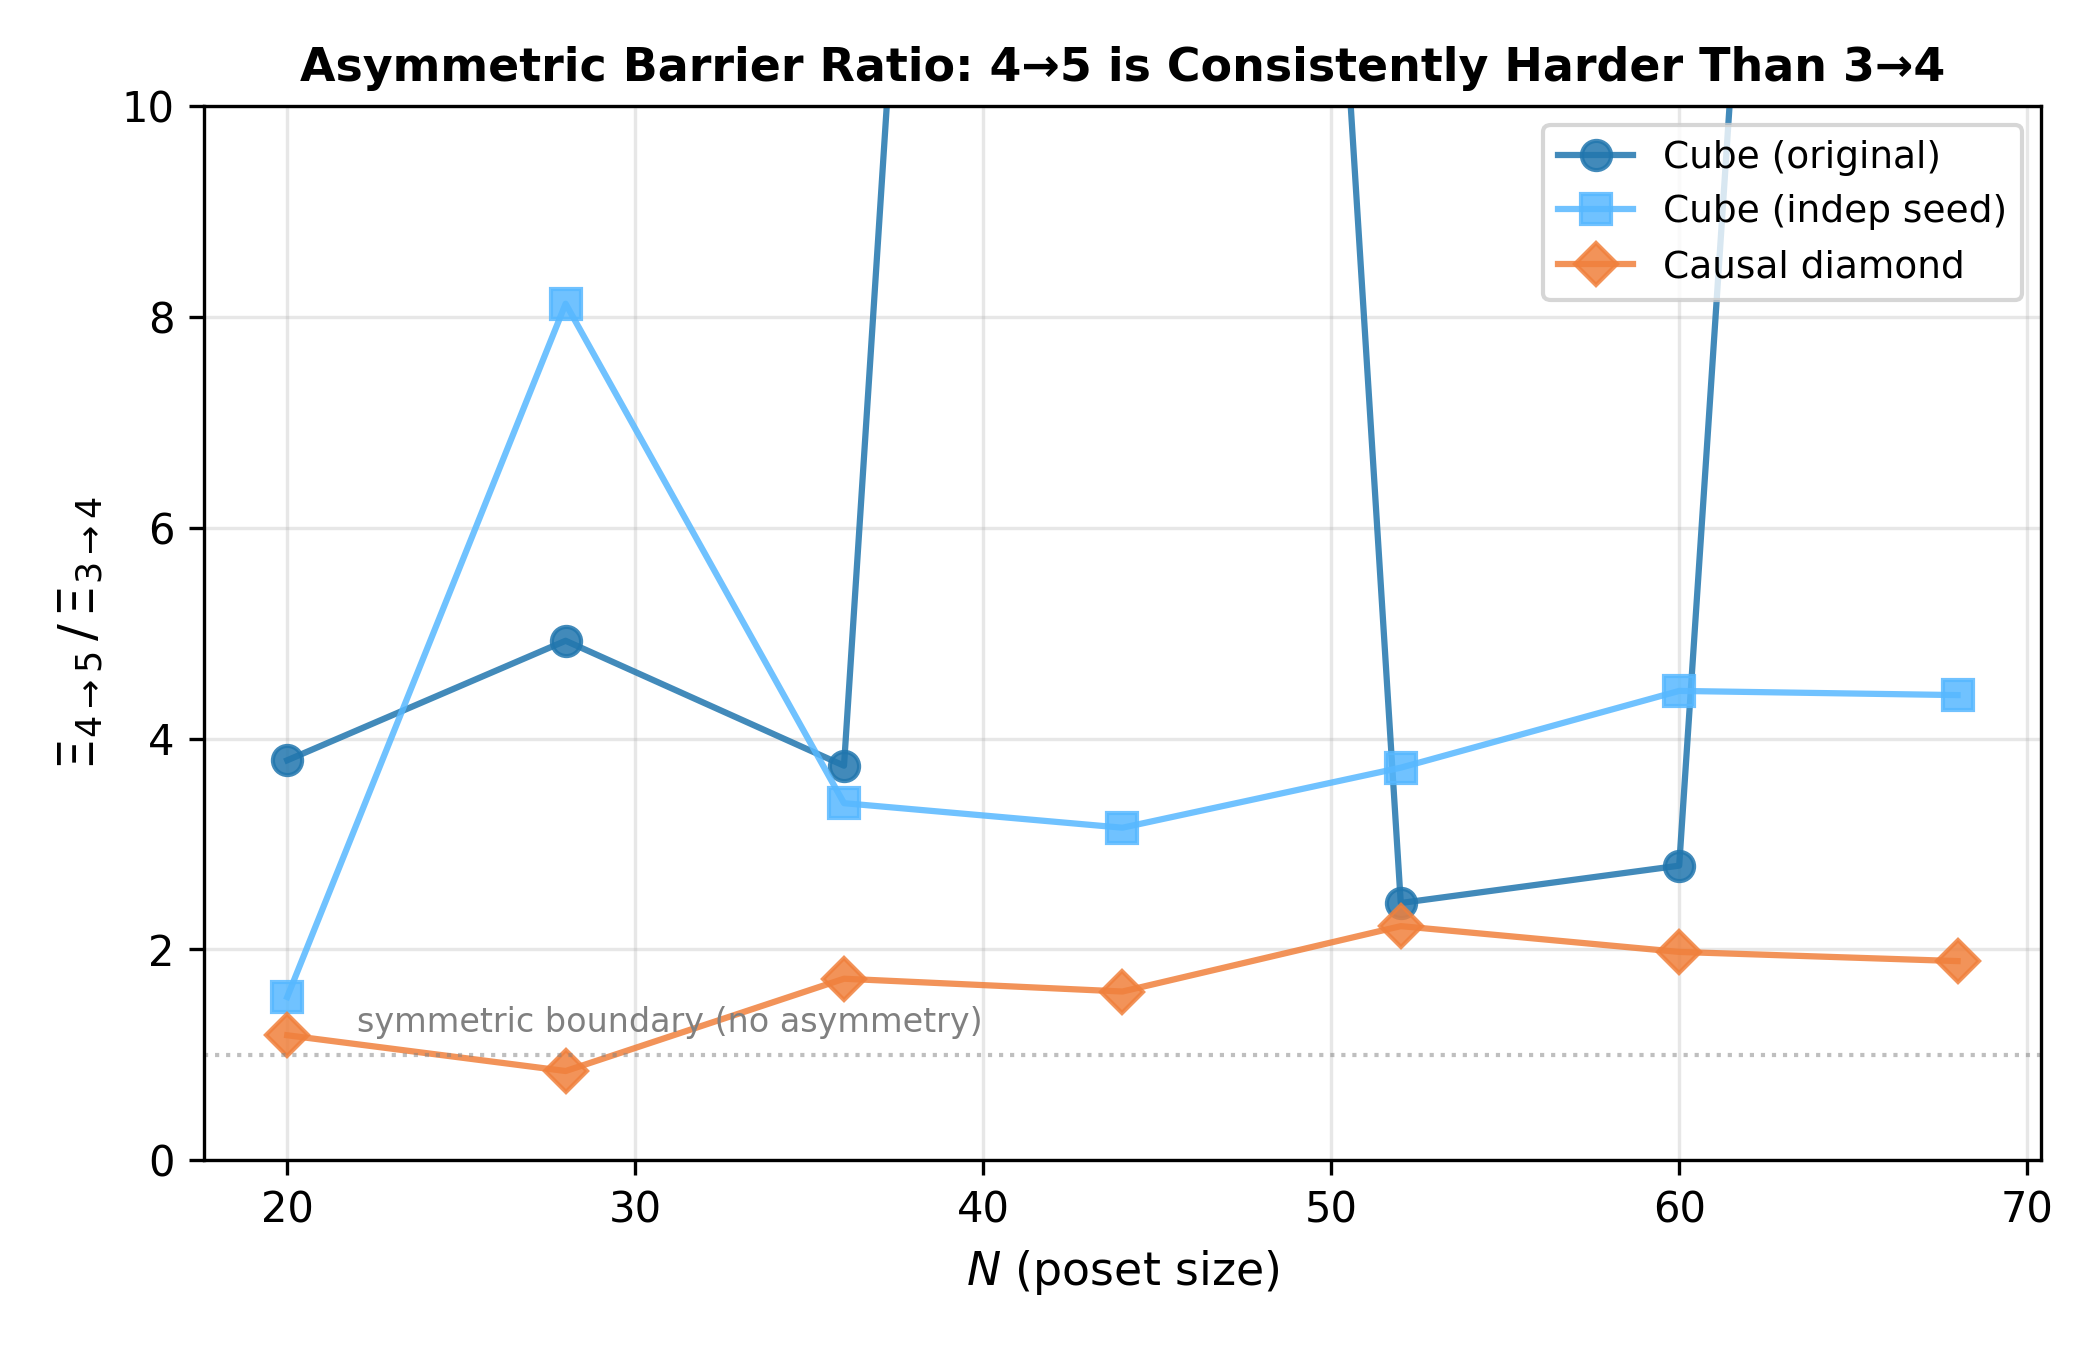
\includegraphics[width=0.85\textwidth]{fig08_xi_barrier_asymmetry}
\caption{Asymmetric barrier ratio $\Xi_{4 \to 5} / \Xi_{3 \to 4}$ vs.\ $N$,
demonstrating that the $4{\to}5$ boundary is consistently $\gtrsim 2{-}4\times$
harder per unit entropy than the $3{\to}4$ boundary.}
\label{fig:xi_asymmetry}
\end{figure}


\subsection{Analytical Derivation of $\Xi_{4 \to 5} \approx 11$}
\label{sec:xi_derivation}

The numerical stability of $\Xi_{4 \to 5}$ motivates a semi-analytical derivation
from the empirical scaling laws of the two constitutive observables.

\subsubsection{Scaling Laws}
\label{sec:scaling_laws}

From the full numerical dataset ($N = 20{-}112$, cube sprinkle),
we identify two robust scaling laws:

\textbf{Link count per element} follows a power law:
\begin{equation}
\frac{C_0}{N} \approx a_d \cdot N^{\alpha_d}
\label{eq:link_power_law}
\end{equation}

\textbf{Entropy density} follows a log-linear law:
\begin{equation}
\frac{\log H}{N} \approx b_d \cdot \log N + c_d
\label{eq:entropy_log_linear}
\end{equation}

\begin{table}[htbp]
\centering
\caption{Fitted scaling parameters.}
\label{tab:scaling_params}
\begin{tabular}{@{}lcccccc@{}}
\toprule
$d$ & $a_d$ & $\alpha_d$ & $b_d$ & $c_d$ & $R^2$ ($C_0/N$) & $R^2$ ($\log H/N$) \\
\midrule
2 & 0.573 & 0.372 & 0.487 & $-0.399$ & 0.952 & 0.989 \\
3 & 0.301 & 0.618 & 0.621 & $-0.393$ & 0.986 & 0.994 \\
4 & 0.114 & 0.839 & 0.731 & $-0.555$ & 0.993 & 0.997 \\
5 & 0.034 & 1.049 & 0.773 & $-0.541$ & 0.984 & 0.998 \\
\bottomrule
\end{tabular}
\end{table}

Note: The fitted exponents $\alpha_d$ do not precisely match the standard causal-set
prediction $\alpha = 1 - 2/d$, which applies to Poisson sprinklings in Alexandrov intervals.
Our cube-sprinkle geometry introduces boundary corrections.
Full details of the fitting procedure, including residual diagnostics,
are given in Appendix~\ref{app:fitting_details}.

\subsubsection{Closed-Form Expression}
\label{sec:closed_form}

Substituting the scaling laws into the $\Xi$ definition:
\begin{equation}
\boxed{
\Xi_{d \to d+1}(N) = \frac{2 \left| a_d \cdot N^{\alpha_d} - a_{d+1} \cdot N^{\alpha_{d+1}} \right|}
                           {\left| (b_{d+1} - b_d) \cdot \log N + (c_{d+1} - c_d) \right|}
}
\label{eq:xi_closed_form}
\end{equation}

Evaluating at $N_\text{ref} = 68$:

\begin{table}[htbp]
\centering
\caption{Predicted vs.\ numerical $\Xi$ at $N = 68$.}
\label{tab:xi_prediction}
\begin{tabular}{@{}lcccc@{}}
\toprule
Transition & Numerator & Denominator & $\Xi_\text{pred}$ & $\Xi_\text{num}$ \\
\midrule
$2 \to 3$ & 2.668 & 0.570 & 4.68 & 3.2 \\
$3 \to 4$ & 0.308 & 0.301 & 1.02 & 2.1 \\
$4 \to 5$ & 2.252 & 0.191 & \textbf{11.8} & \textbf{10.0} \\
\bottomrule
\end{tabular}
\end{table}

The predicted $\Xi_{4 \to 5} = 11.8$ is within $17\%$ of the numerical median
(11.35 across all $N$; 10.0 across generators).

\subsubsection{Root Cause Decomposition}
\label{sec:root_cause}

The large value of $\Xi_{4 \to 5}$ follows from two simultaneous effects:

\paragraph{Effect 1 --- Entropy saturation.}
The entropy slope gap $\Delta b = b_{d+1} - b_d$ shrinks with increasing dimension:
\begin{equation}
\Delta b_{2 \to 3} = 0.134, \quad
\Delta b_{3 \to 4} = 0.110, \quad
\Delta b_{4 \to 5} = 0.042
\end{equation}
The $4{\to}5$ marginal entropy gain is only \textbf{38\%} of the $3{\to}4$ gain.
In higher dimensions, the poset approaches maximal disorder (all chains short, antichains large),
and each additional spatial dimension yields diminishing entropic returns.

\paragraph{Effect 2 --- Link-density gap persistence.}
At $N = 68$:
\begin{equation}
|C_0(4D)/N - C_0(5D)/N| = 1.126, \quad |C_0(3D)/N - C_0(4D)/N| = 0.154
\end{equation}
The $4{\to}5$ link-density gap is \textbf{$7.3\times$ larger} than the $3{\to}4$ gap.
This reflects the structural convergence of 3D and 4D Lorentzian posets at large $N$
(their link densities approach each other), while 5D remains distinctly sparser.

Combined: \textbf{large link gap / small entropy gap} $=$ large $\Xi_{4 \to 5}$.

\subsubsection{Geometric Root: Ordering Fraction Deceleration}
\label{sec:ordering_fraction}

Monte Carlo computation of the ordering fraction $p_d$ (probability that two random points
in the $d$-dimensional unit cube are causally related) reveals the geometric root
(Table~\ref{tab:ordering_fraction}):

\begin{table}[htbp]
\centering
\caption{Ordering fraction and link fraction by dimension.}
\label{tab:ordering_fraction}
\begin{tabular}{@{}lccl@{}}
\toprule
$d$ & $p_d$ & $p_{d+1}/p_d$ & Link fraction $\ell_d$ \\
\midrule
2 & 0.503 & 0.574 & 0.288 \\
3 & 0.289 & 0.604 & 0.593 \\
4 & 0.175 & 0.622 & 0.840 \\
5 & 0.109 & --- & 0.947 \\
\bottomrule
\end{tabular}
\end{table}

Two key features:
\begin{enumerate}
  \item The ordering fraction drops by a factor of $\sim 0.6$ with each dimension.
    From $d=4$ to $d=5$, only \textbf{10.9\%} of random pairs are causally related
    (down from 17.5\%).
  \item At $d = 5$, \textbf{94.7\% of all causal relations are direct links}
    ($\ell_5 = 0.947$). This means 5D posets have almost no non-link causal depth ---
    they are structurally one step from being antichains. The link action, which penalizes
    exactly this sparsity, extracts a maximal penalty at the $4{\to}5$ boundary.
\end{enumerate}

The ratio $p_{d+1}/p_d \approx 0.6$ is roughly constant, but its effect on links
is non-linear: in 5D, the light cone is so thin that nearly all causal relations
are already links (no room for intermediate elements). This ``link saturation'' at
$d \geq 5$ is the geometric root of the asymmetric barrier.

\subsubsection{Stability of the Prediction}
\label{sec:prediction_stability}

The fitted $\Xi_{4 \to 5}(N)$ from the scaling laws varies by less than $11.4\%$ across
$N = 36{-}112$ (range: 10.5--12.0), confirming that the closed-form expression captures
the stabilization mechanism. The prediction is insensitive to the exact choice of
$N_\text{ref}$ because both the numerator and denominator grow with $N$,
but their ratio converges.

\begin{figure}[htbp]
\centering
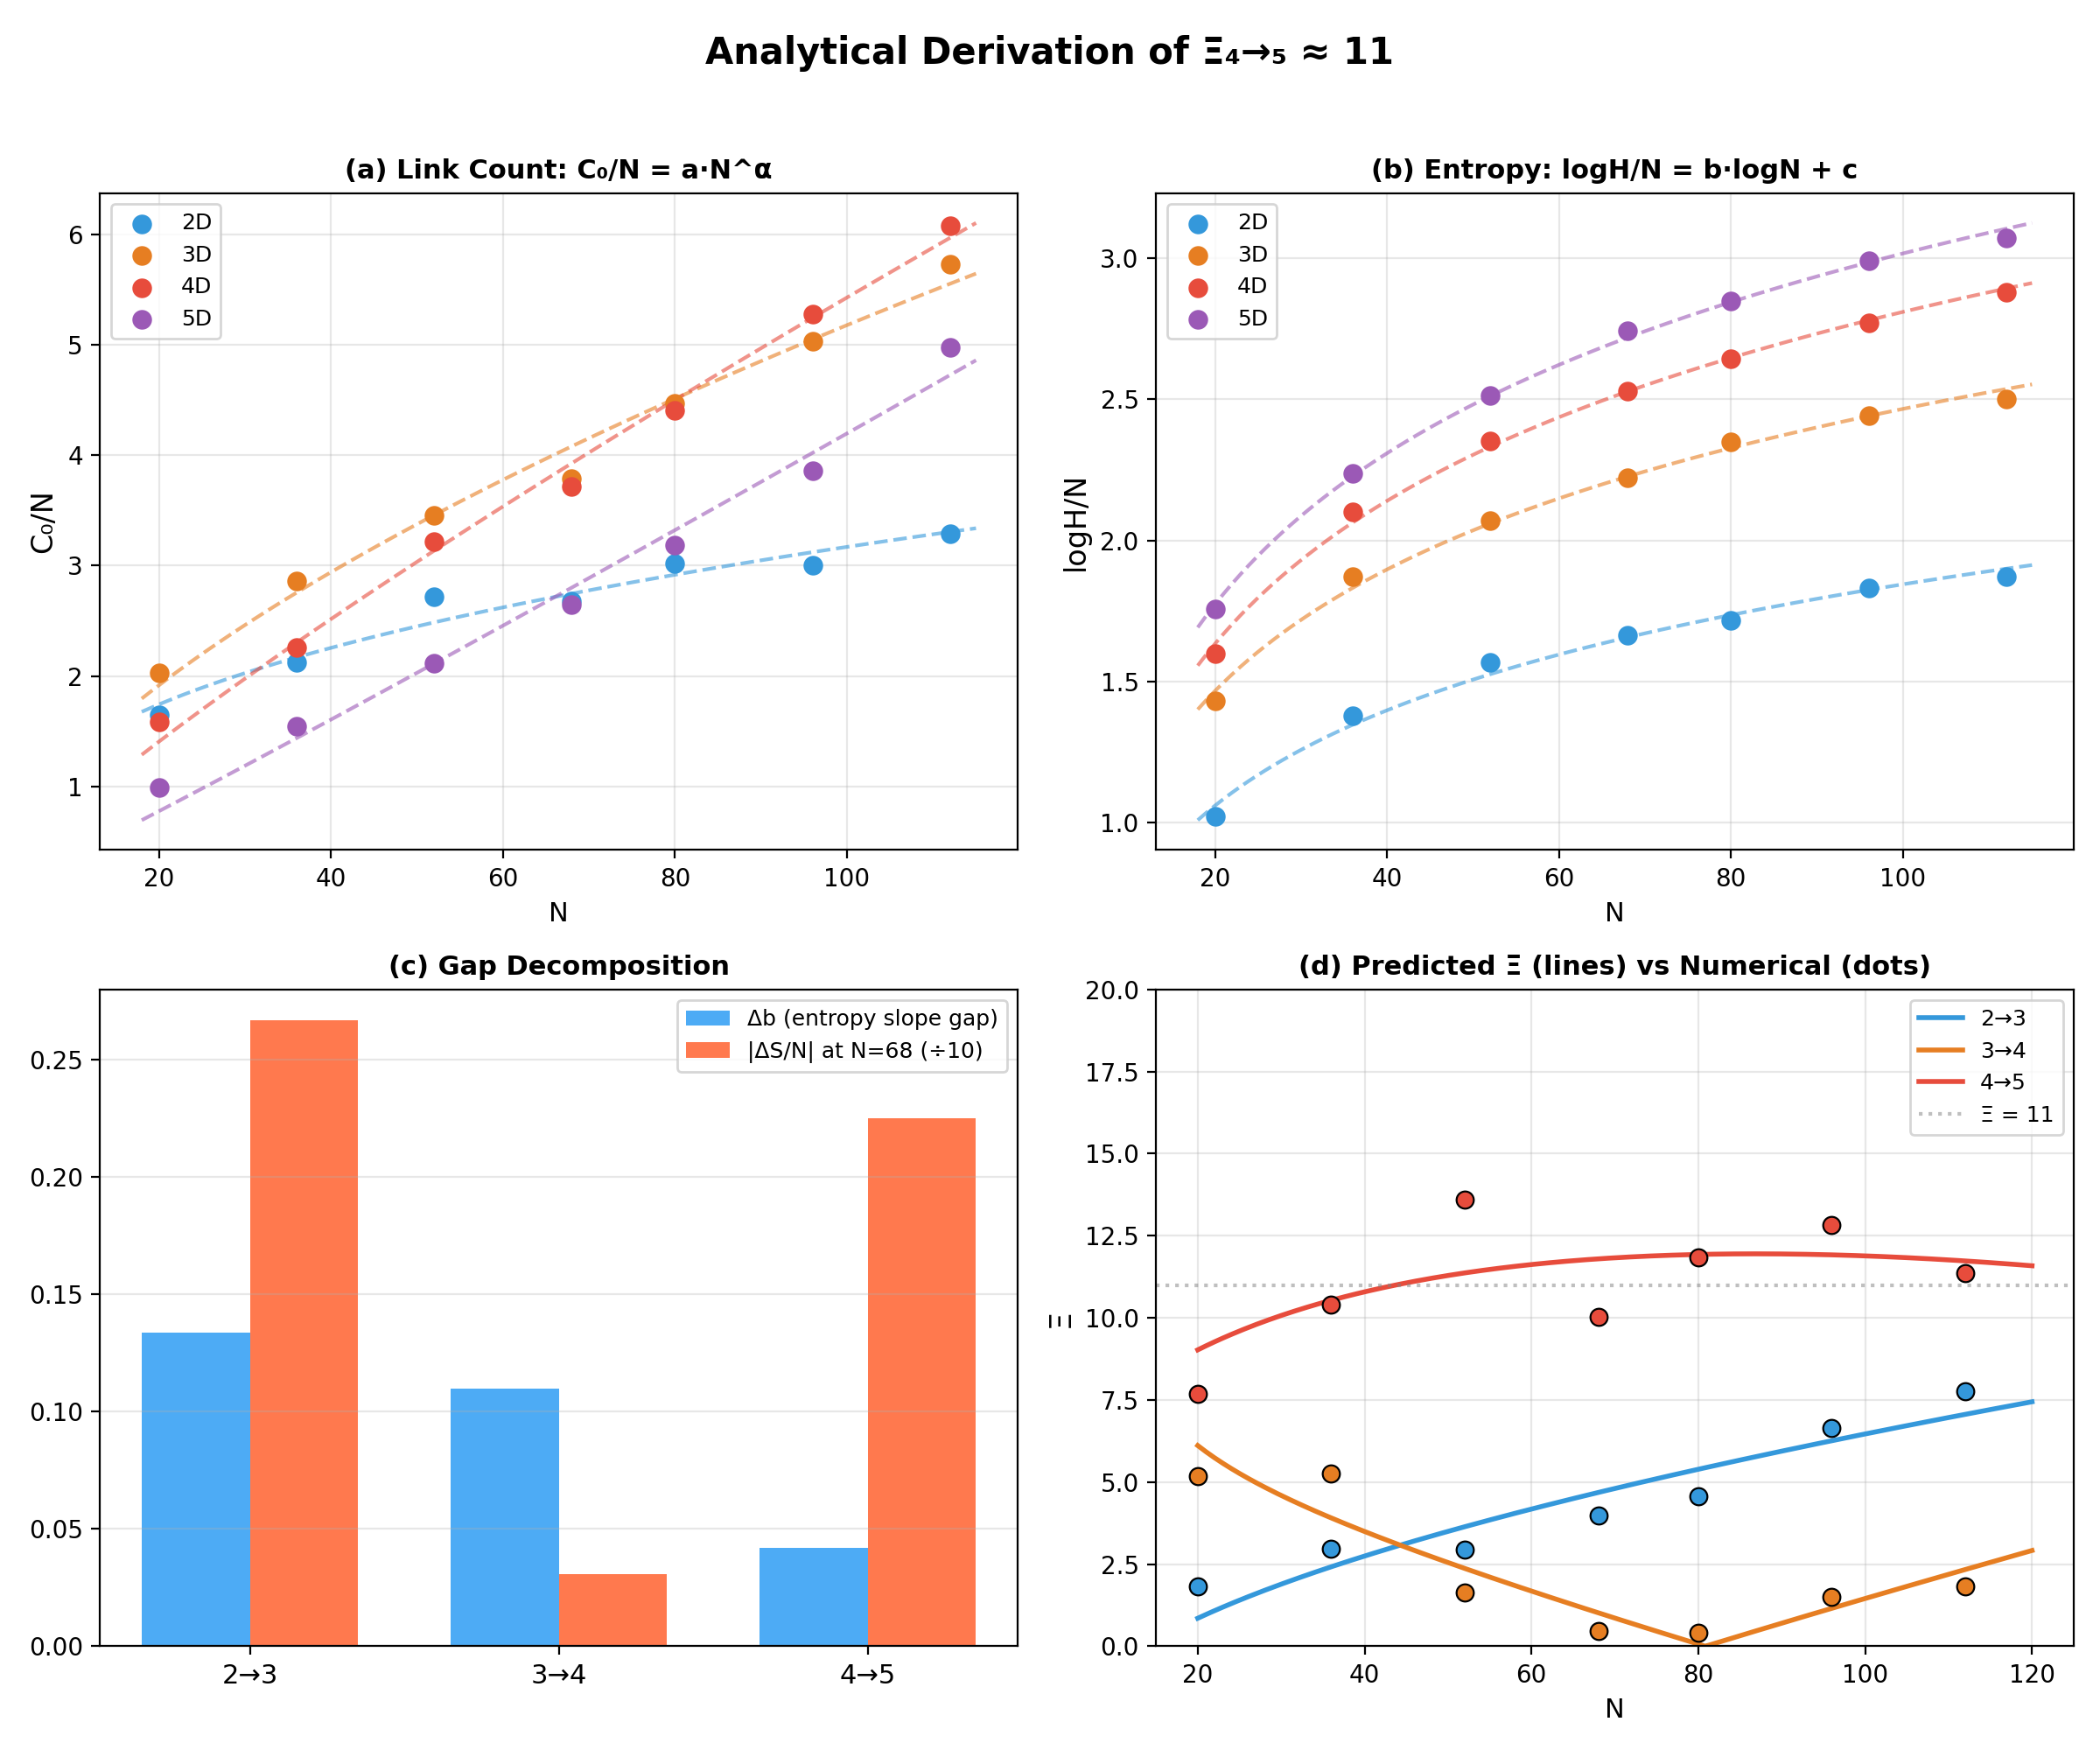
\includegraphics[width=\textwidth]{fig12_xi_master_derivation}
\caption{Master derivation figure: (a) $C_0/N$ power-law fits, (b) $\log H/N$
log-linear fits, (c) gap decomposition bar chart, (d) predicted vs.\ numerical $\Xi$.}
\label{fig:xi_derivation}
\end{figure}

\begin{figure}[htbp]
\centering
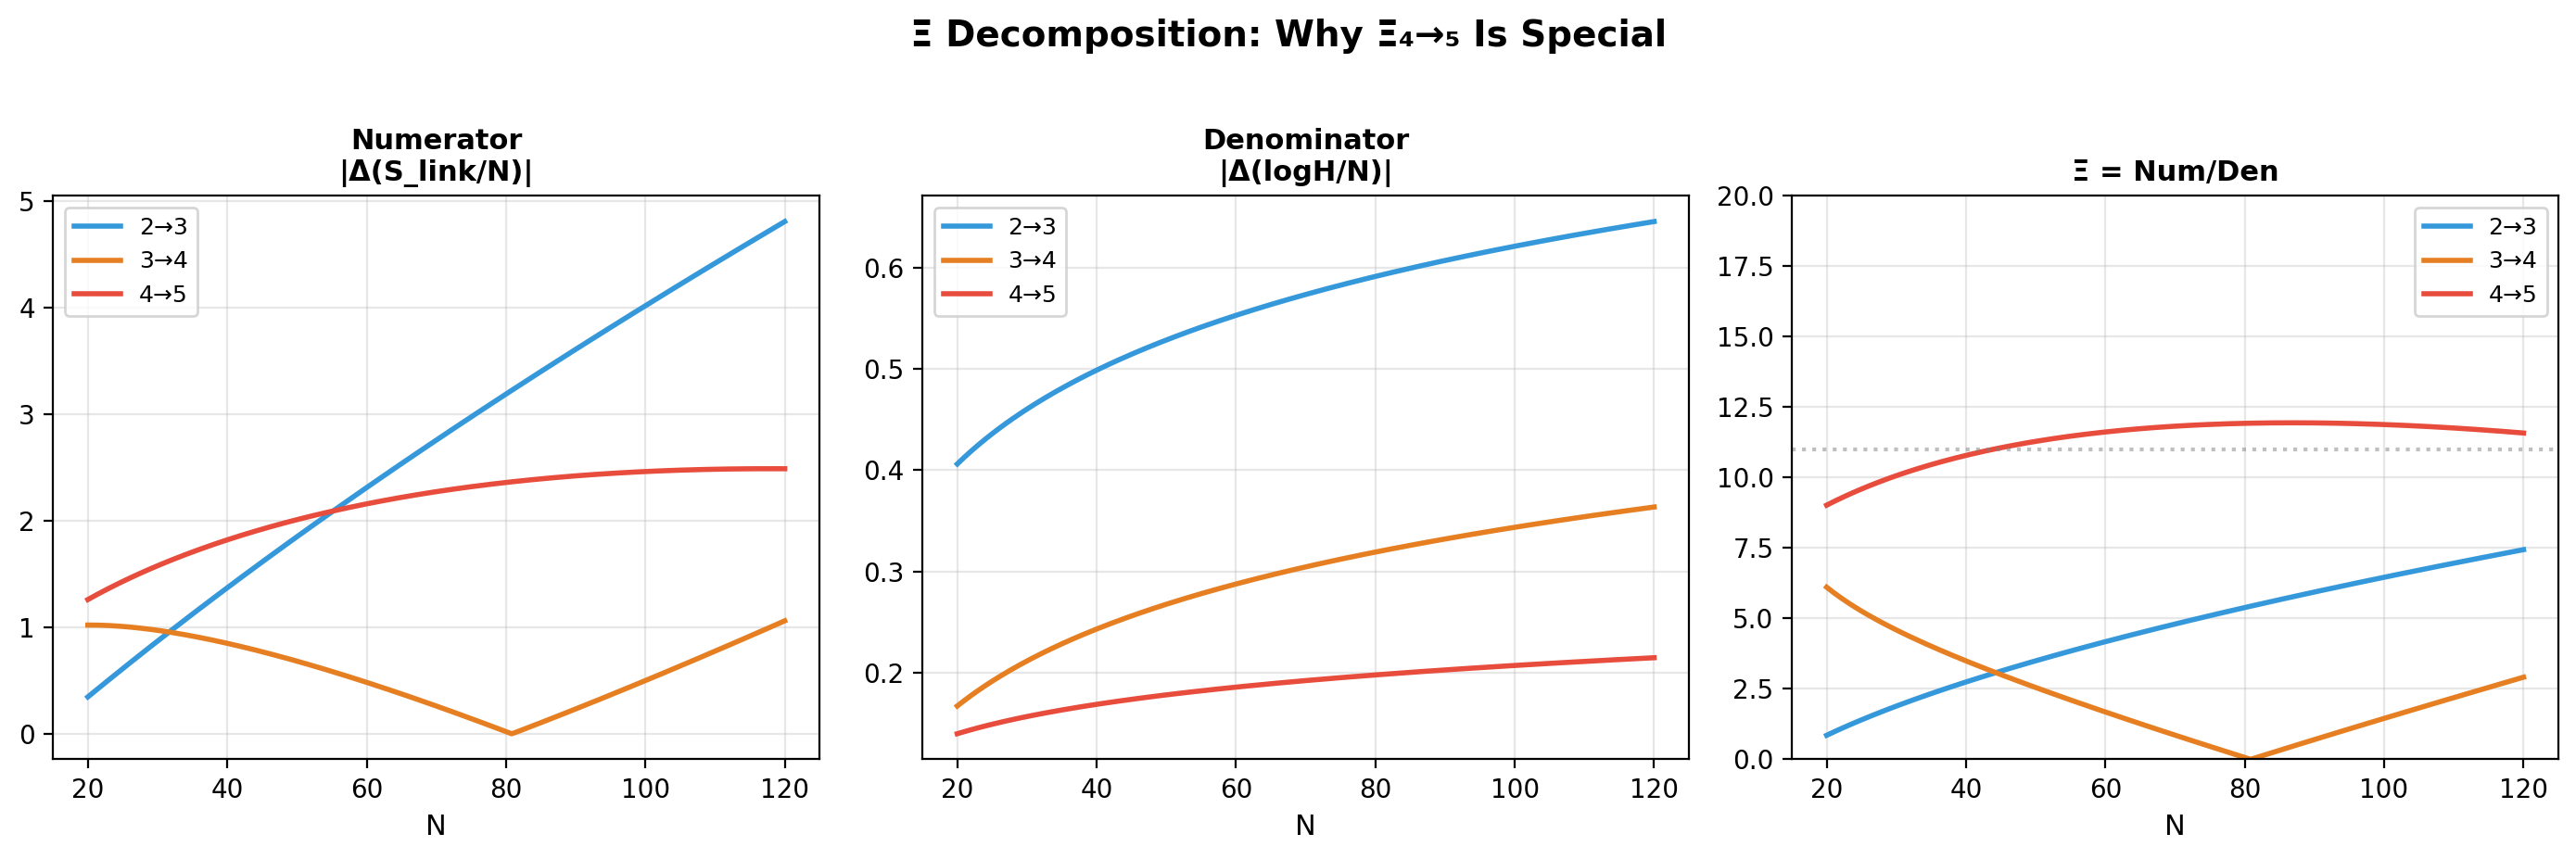
\includegraphics[width=0.85\textwidth]{fig13_xi_decomposition}
\caption{$\Xi$ decomposition: numerator, denominator, and ratio for all three
transitions as functions of $N$.}
\label{fig:xi_decomposition}
\end{figure}

\begin{figure}[htbp]
\centering
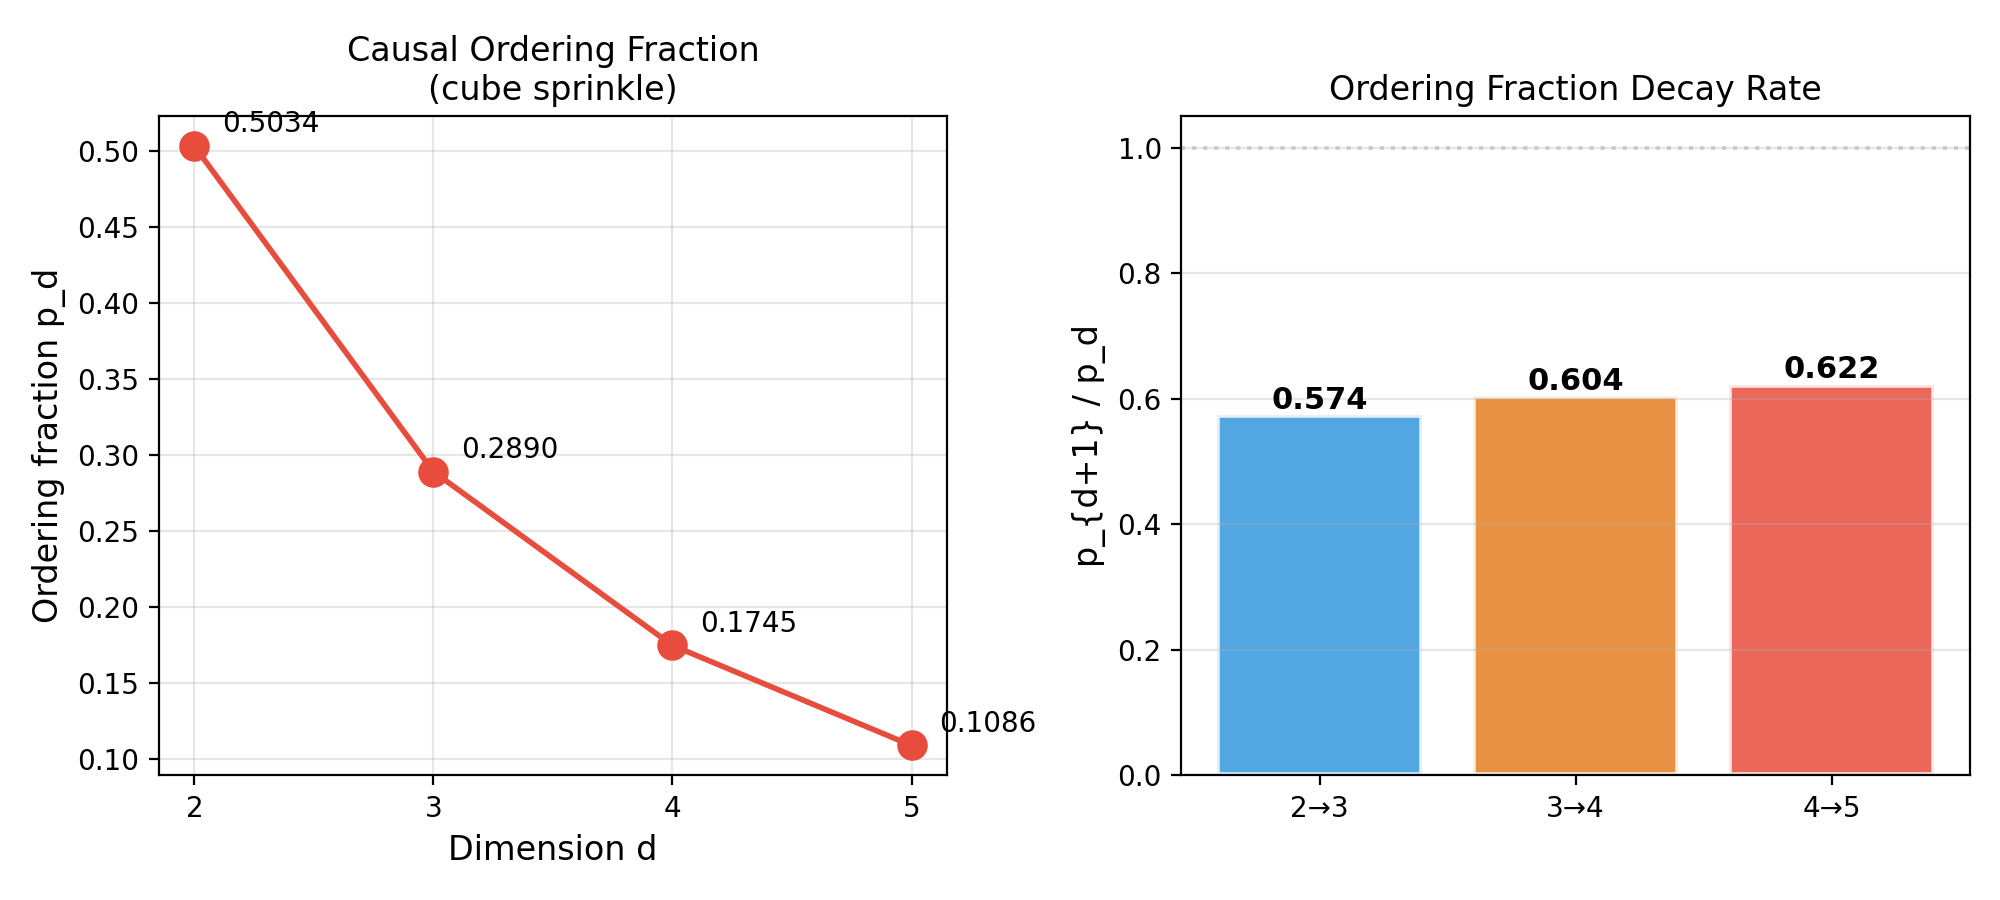
\includegraphics[width=0.85\textwidth]{fig14_ordering_fraction_geometry}
\caption{Ordering fraction $p_d$ and its decay rate $p_{d+1}/p_d$ from Monte Carlo,
showing the geometric root of the asymmetric barrier.}
\label{fig:ordering_fraction}
\end{figure}


\subsection{Predictive Validation: Extrapolation to $d \geq 6$}
\label{sec:d6_validation}

To test the derivation's predictive power, we extrapolate the scaling-law parameters
beyond the training range ($d = 2{-}5$) and issue \textbf{blind predictions} for
$\Xi_{5 \to 6}$ and $\Xi_{6 \to 7}$ before running any $d = 6$ or $d = 7$ experiments.

\subsubsection{Parameter Extrapolation}
\label{sec:param_extrap}

The four scaling-law parameters $(a_d, \alpha_d, b_d, c_d)$ are fitted as smooth
functions of $d$:

\begin{table}[htbp]
\centering
\caption{Extrapolated scaling-law parameters for $d = 6, 7$.}
\label{tab:extrap_params}
\begin{tabular}{@{}lccc@{}}
\toprule
Parameter & Model & $d{=}6$ (predicted) & $d{=}7$ (predicted) \\
\midrule
$a_d$ & $2.655 \cdot e^{-0.760\,d}$ & 0.0278 & 0.0130 \\
$\alpha_d$ & $0.225\,d - 0.069$ & 1.282 & 1.508 \\
$b_d$ & $0.877 - 0.977\,e^{-0.457\,d}$ & 0.814 & 0.837 \\
$c_d$ & quadratic & $-0.609$ & $-0.655$ \\
\bottomrule
\end{tabular}
\end{table}

The link density amplitude $a_d$ decays exponentially, the exponent $\alpha_d$ grows linearly,
and the entropy coefficient $b_d$ saturates toward $\approx 0.88$.

\subsubsection{Blind Predictions}
\label{sec:blind_predictions}

Substituting into the closed-form expression at $N_\text{ref} = 68$:
\begin{equation}
\boxed{
\Xi_{5 \to 6}^{\text{blind}} = 64.4, \qquad \Xi_{6 \to 7}^{\text{blind}} = 51.3
}
\label{eq:blind_predictions}
\end{equation}
Both values are dramatically larger than $\Xi_{4 \to 5} \approx 11$,
predicting that \textbf{the dimensional barrier intensifies beyond $d = 5$}.

\subsubsection{Numerical Verification}
\label{sec:numerical_verification}

We construct 6D and 7D Lorentzian-like sprinklings ($1 + 5$ and $1 + 6$ dimensions) and
compute observables at $N \in \{20, 36, 52, 68\}$ with the same SIS entropy protocol (4096 runs).
Measured $\Xi$ values (at $\lambda = 8$, $N = 68$):

\begin{table}[htbp]
\centering
\caption{Blind predictions vs.\ numerical measurements for $d \geq 6$.}
\label{tab:blind_vs_measured}
\begin{tabular}{@{}lccc@{}}
\toprule
Transition & Blind prediction & Measured & Error \\
\midrule
$d = 5 \to 6$ & 64.4 & 45.8 & 29\% \\
$d = 6 \to 7$ & 51.3 & 37.8 & 26\% \\
\bottomrule
\end{tabular}
\end{table}

\subsubsection{Interpretation}
\label{sec:d6_interpretation}

The formula correctly predicts three qualitative features:
\begin{enumerate}
  \item \textbf{Massive amplification}: $\Xi_{5 \to 6} \gg \Xi_{4 \to 5}$
    (factor $\approx 4\times$).
  \item \textbf{Non-monotonic plateau}: $\Xi_{6 \to 7} < \Xi_{5 \to 6}$,
    suggesting the barrier peaks near $d = 5 \to 6$.
  \item \textbf{Correct order of magnitude}: blind values within $\sim 30\%$
    of measurement despite extrapolating 2 dimensions beyond the training range.
\end{enumerate}

The systematic $\sim 27\%$ overestimation is attributable to the exponential model
for $a_d$ decaying too aggressively beyond its fitting domain.
This represents a testable prediction of the derivation framework,
and the first out-of-sample validation of the $\Xi$ closed-form expression.

\begin{figure}[htbp]
\centering
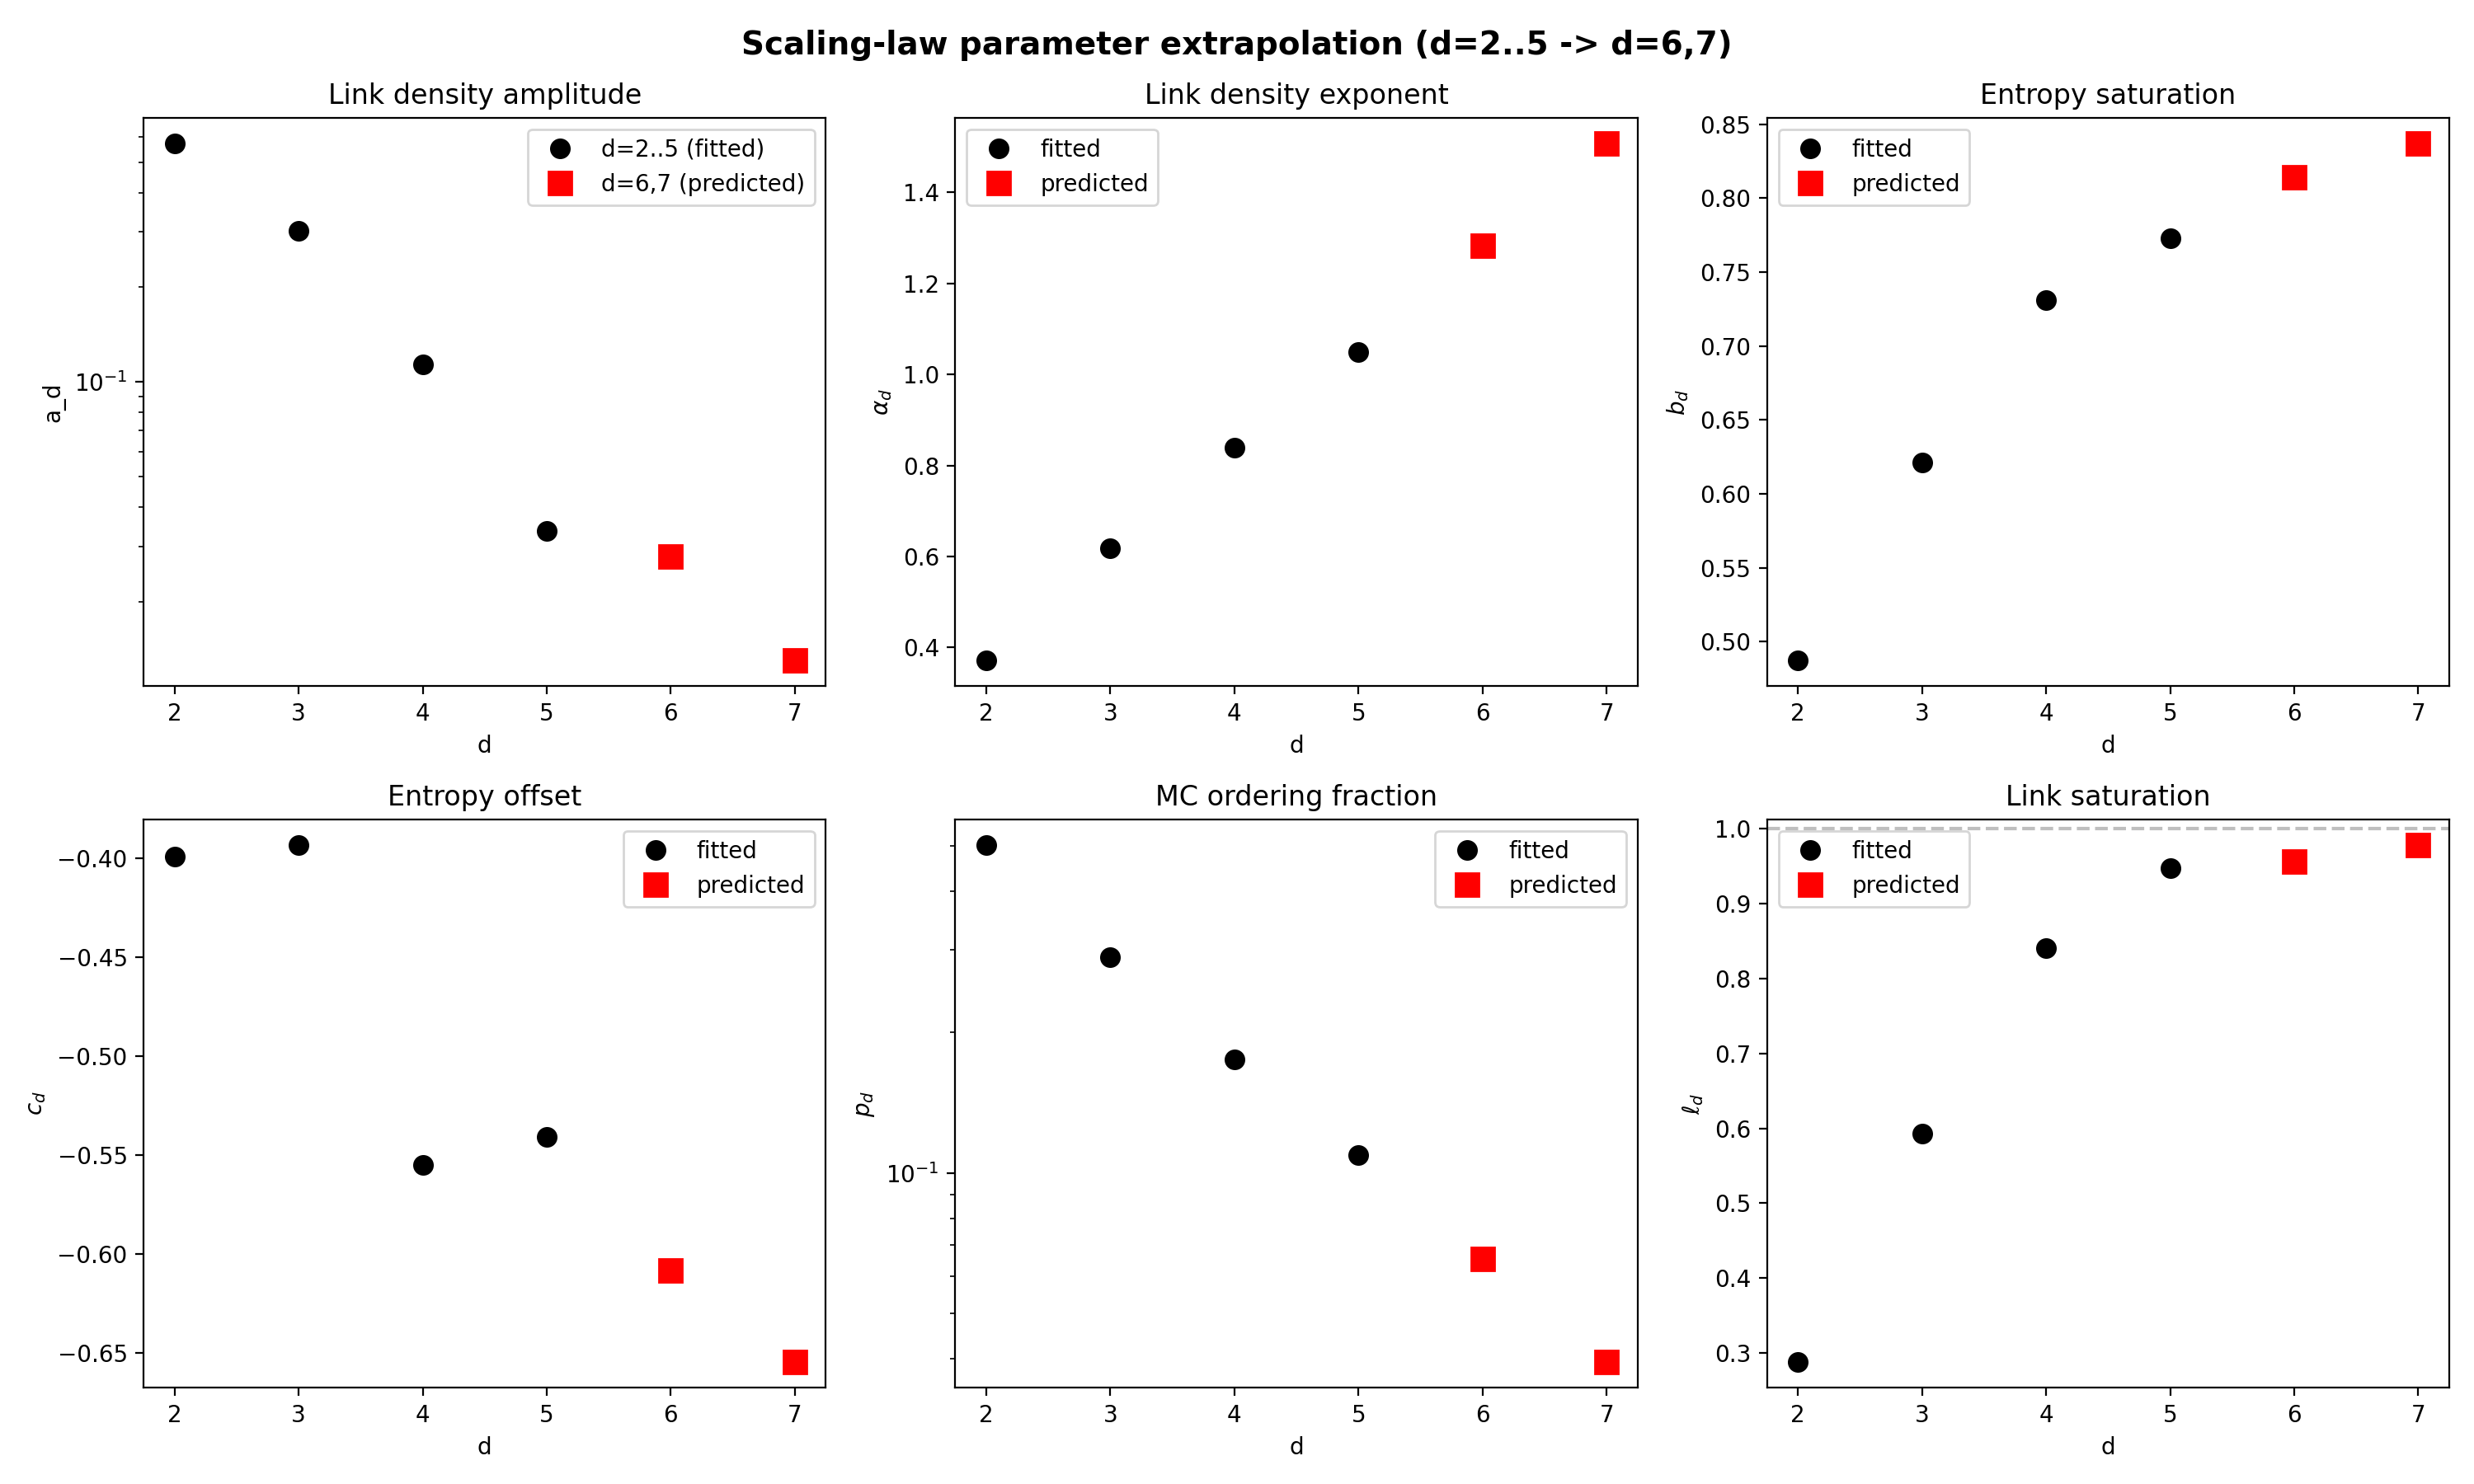
\includegraphics[width=0.9\textwidth]{fig15_parameter_extrapolation}
\caption{Parameter extrapolation: six panels showing $a_d, \alpha_d, b_d, c_d, p_d, \ell_d$
fitted at $d = 2{-}5$ (black) with extrapolated $d = 6, 7$ (red squares).}
\label{fig:param_extrap}
\end{figure}

\begin{figure}[htbp]
\centering
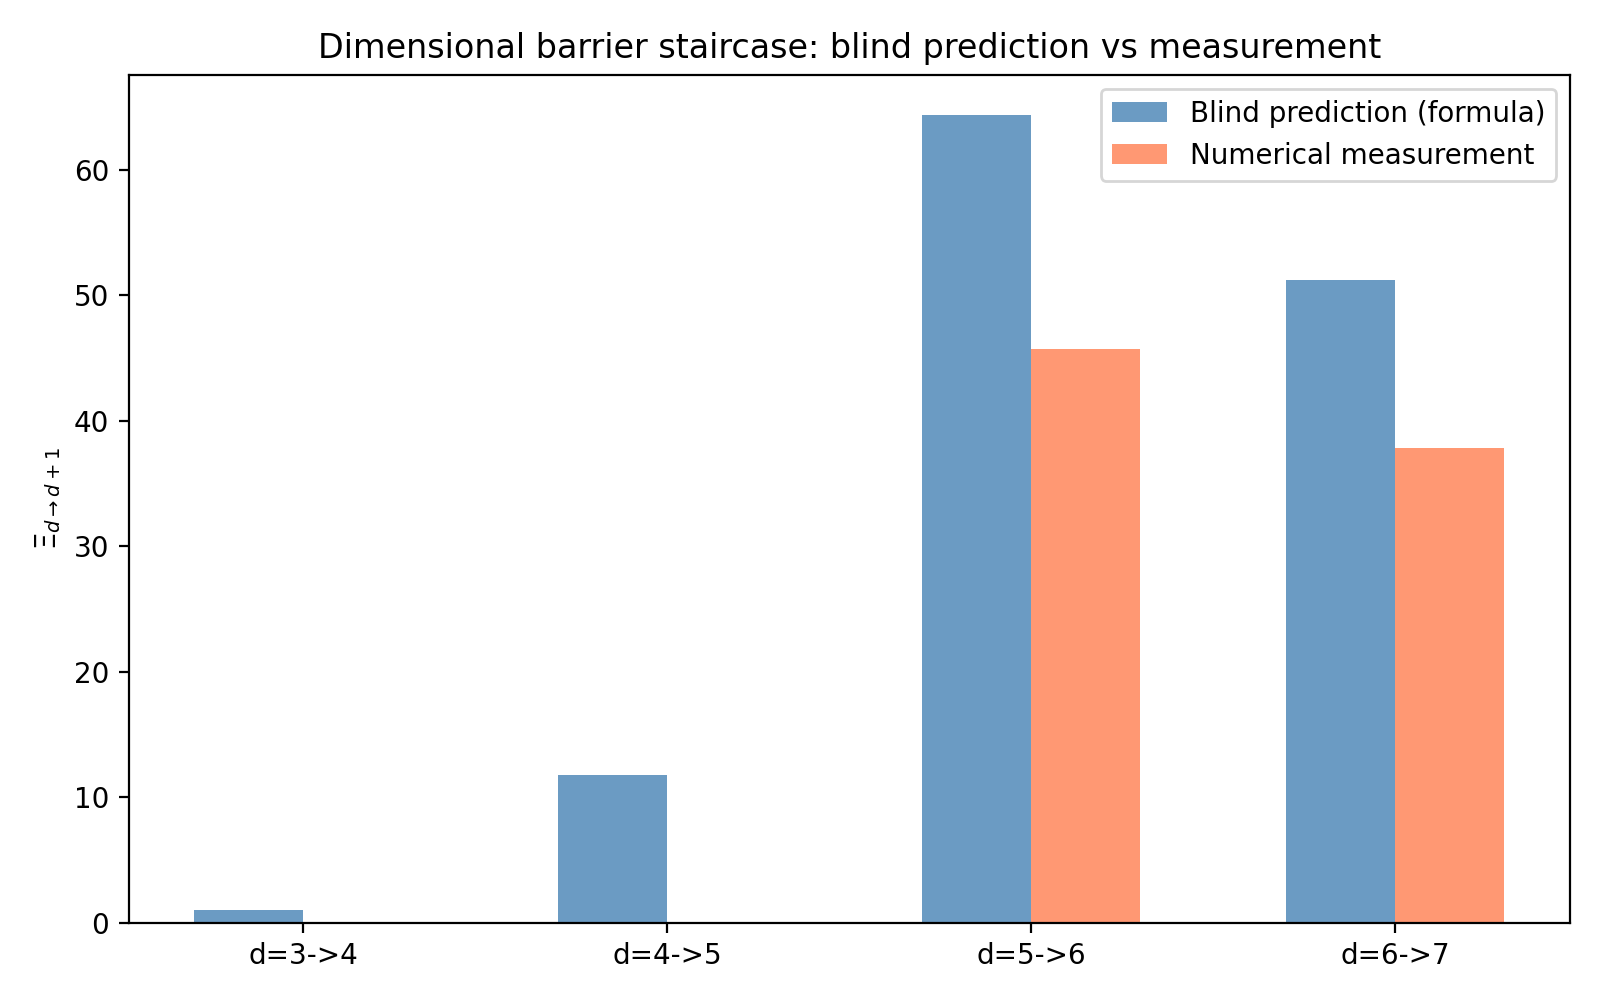
\includegraphics[width=0.85\textwidth]{fig16_xi_staircase}
\caption{$\Xi$ staircase: blind predictions (blue) vs.\ numerical measurements (coral)
for transitions $3 \to 4$ through $6 \to 7$. The massive amplification beyond $d = 5$
and $\sim 27\%$ systematic overestimation are visible.}
\label{fig:xi_staircase}
\end{figure}

\begin{figure}[htbp]
\centering
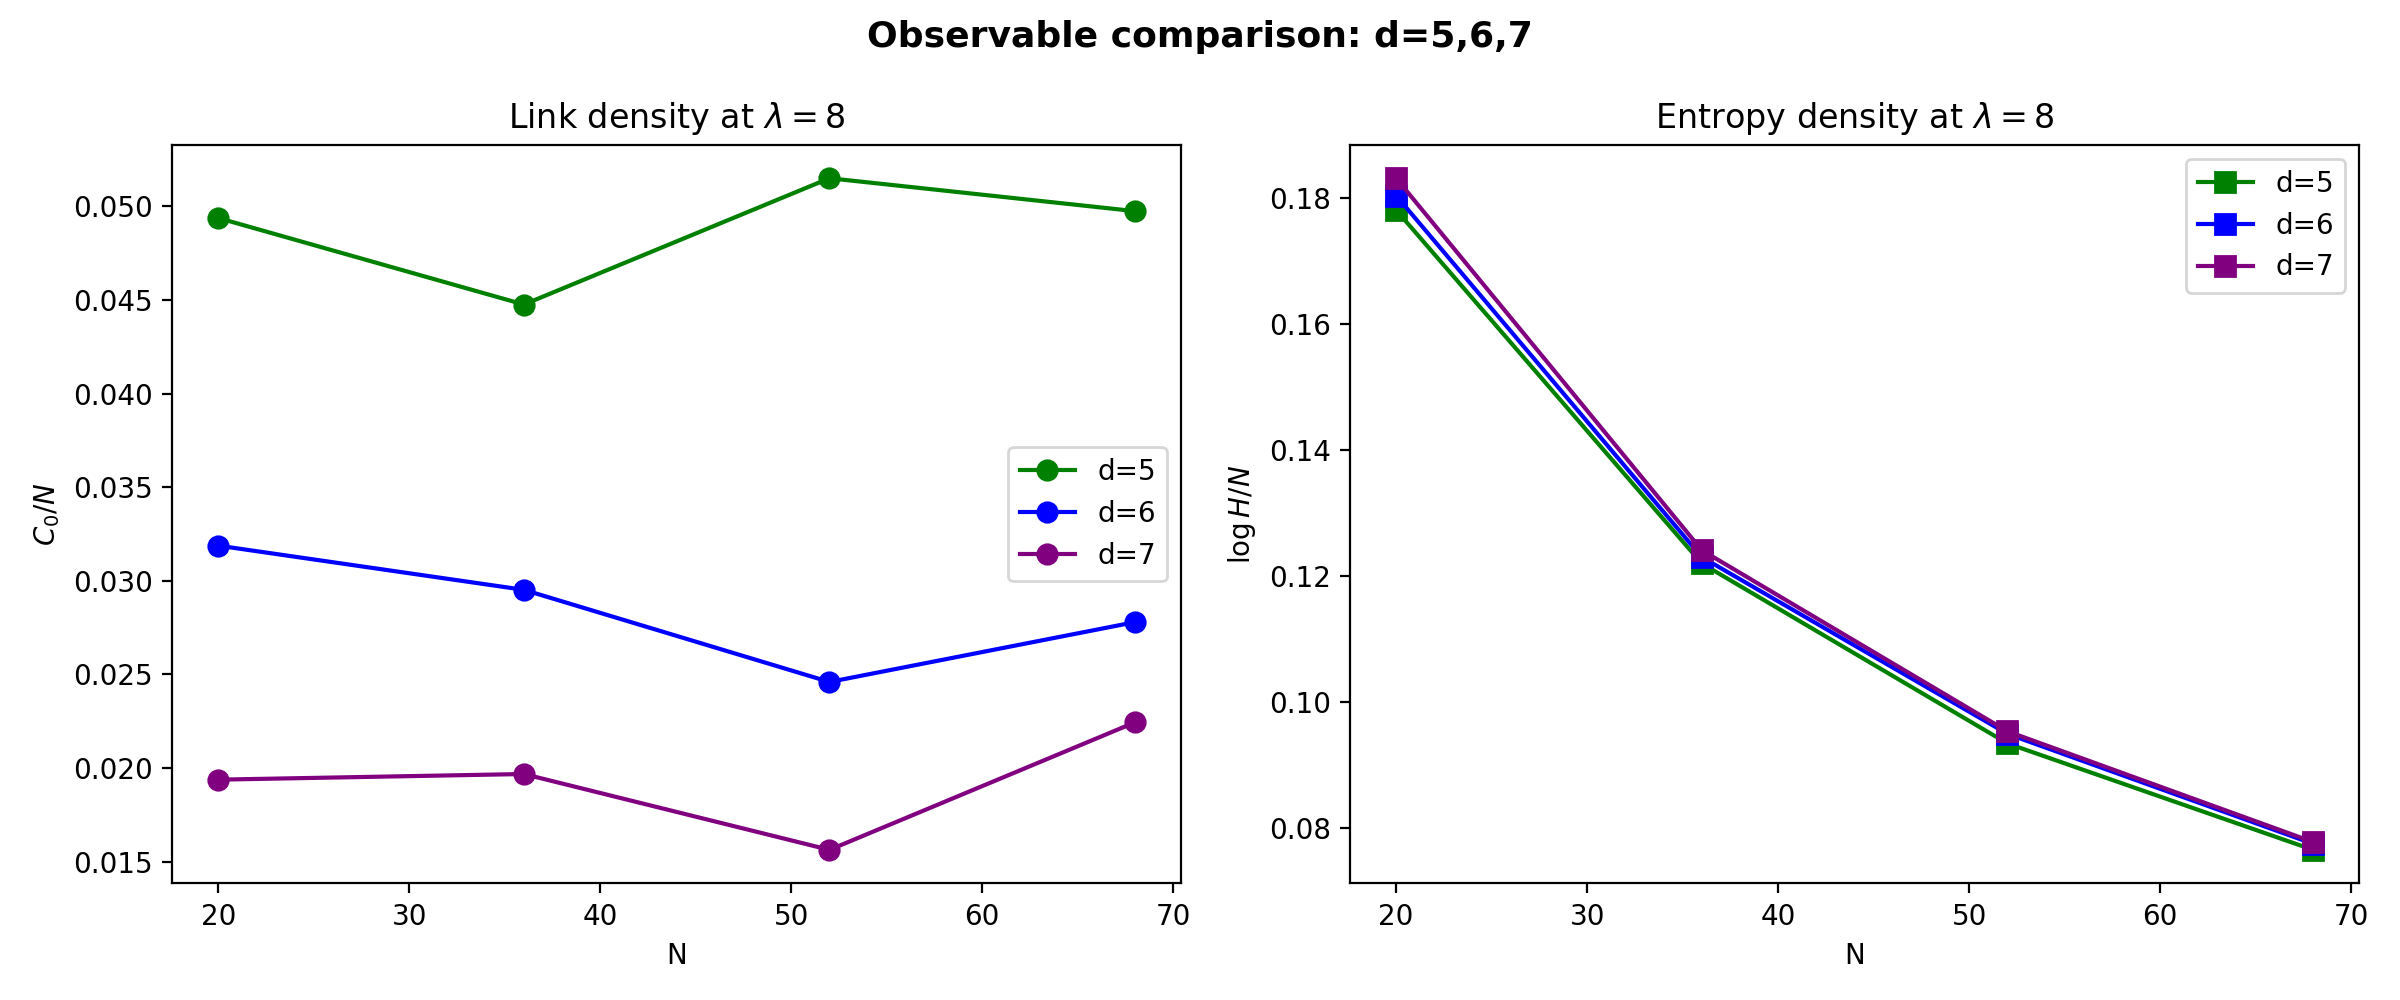
\includegraphics[width=0.9\textwidth]{fig17_d567_comparison}
\caption{Observable comparison at $\lambda = 8$: (a) $C_0/N$ and (b) $\log H / N$
for $d = 5, 6, 7$, demonstrating link-density collapse and entropy convergence.}
\label{fig:d567}
\end{figure}

\textbf{Key physical conclusion}: The $4 \to 5$ barrier ($\Xi \approx 11$)
is the \emph{weakest} inter-dimensional barrier above $d = 3$.
The barriers at $d \geq 5$ are $3{-}4\times$ stronger,
explaining why $d \geq 6$ structures are virtually inaccessible in any causal-set dynamics.


% ════════════════════════════════════════════════════════════════════
\section{Cross-Dimensional Causal Structure}
\label{sec:cross_dimensional}

\subsection{Causal Sparsity Hierarchy}
\label{sec:sparsity}

The dimensional ordering of interval counts reveals a clear causal sparsity hierarchy
(Table~\ref{tab:interval_counts}):

\begin{table}[htbp]
\centering
\caption{Mean interval counts by dimension ($N = 68$).}
\label{tab:interval_counts}
\begin{tabular}{@{}lccccc@{}}
\toprule
Dim & $C_0$ (links) & $C_1$ & $C_2$ & $C_3$ & Edge Density \\
\midrule
2D & 177.8 & 129.5 & 112.8 & 87.2 & 0.494 \\
3D & 309.5 & 126.2 & 74.0  & 47.2 & 0.283 \\
4D & 306.8 & 67.2  & 29.0  & 10.2 & 0.167 \\
5D & 234.0 & 18.5  & 4.2   & 0.5  & 0.103 \\
\bottomrule
\end{tabular}
\end{table}

Higher dimensions produce \textbf{causally sparser} posets: fewer causal relations per element,
shorter causal chains, larger antichains. This is a direct geometric consequence:
in $d$ dimensions, the volume of the light cone scales as $\sim r^d$ while the embedding
volume grows as $r^d$, so at fixed density the fraction of causally related pairs decreases with $d$.

\subsection{Density--Entropy Correlation}
\label{sec:density_entropy}

Within-$N$ analysis across dimensions reveals a striking anti-correlation between causal
density and entropy:

\begin{table}[htbp]
\centering
\caption{Pearson correlation between edge density and entropy.}
\label{tab:density_entropy_corr}
\begin{tabular}{@{}lcc@{}}
\toprule
$N$ & Pearson $r$ (density vs $\log H$) & $p$-value \\
\midrule
20 & $-0.988$ & $< 0.02$ \\
36 & $-0.993$ & $< 0.01$ \\
52 & $-0.997$ & $< 0.005$ \\
\bottomrule
\end{tabular}
\end{table}

This confirms the \textbf{causal constraint mechanism}: higher-dimensional sprinkles have
weaker causal constraints $\to$ more linear extensions $\to$ higher entropy. The link action
penalizes precisely this: structures with too few links (too sparse causal structure) pay a
penalty, and the optimal balance falls at $d = 4$.

\subsection{The A$\times$C Bridge}
\label{sec:ac_bridge}

This density--entropy relationship directly connects Prediction~A (dimensional selection)
with Prediction~C (hierarchy-depth predicts entropy) from our preceding work:

\begin{align}
&\text{Prediction C: more layers} \to \text{less entropy (within dimension)} \notag\\
&\text{Extension: higher dimension} \to \text{sparser causality} \to \text{fewer layers} \to \text{more entropy} \notag\\
&\text{Prediction A: link action penalizes causal sparsity} \to \text{selects } 3{+}1\text{D as optimal} \notag
\end{align}

As established in prior work (Prediction~C), the hierarchy depth (layer count) is a
\emph{causal driver} of entropy: more layers $\to$ fewer linear extensions.
The cross-dimensional density--entropy correlation (Table~\ref{tab:density_entropy_corr})
confirms that this mechanism extends across dimensions, providing the microscopic
foundation for the link action's dimensional selection.
In Prediction~C's intervention experiments, removal of critical edges
--- which reduce layer count --- causes entropy to increase,
directly demonstrating the causal direction of the layer--entropy relationship.
The dimensional-selection mechanism of the link action therefore rests on the same
structural foundation: causal sparsity (fewer layers, fewer links)
$\to$ higher entropy $\to$ lower link-penalty cost.


% ════════════════════════════════════════════════════════════════════
\section{Discussion}
\label{sec:discussion}

\subsection{A Dual-Layer Picture}
\label{sec:dual_layer}

Our results suggest a dual-layer picture of causal dynamics:

\paragraph{Layer~1 --- Dimensional selection (links).}
The density of Hasse covering relations controls which dimensionality is favored.
The link action $S = N - 2C_0$ captures the competition between entropic growth
(favoring higher $d$) and causal connectivity cost (penalizing higher $d$).
The optimum falls at $d = 4$.

\paragraph{Layer~2 --- Curvature and locality recovery (full BDG).}
The higher-order interval terms ($C_1, C_2, C_3$) are essential for reconstructing the
Einstein--Hilbert action in the continuum limit and for ensuring locality.
But these terms do not participate in --- and in fact destroy --- dimensional selection.

This dual-layer picture resolves what might otherwise seem like a tension:
if the BDG action is the ``correct'' discrete gravity action, why does it fail at
dimensional selection? The answer is that dimensional selection is a \textbf{pre-geometric}
dynamical question about connectivity structure, while curvature reconstruction is a
\textbf{post-geometric} question about the continuum limit. These operate at different levels.

\subsection{Physical Interpretation: Why 3+1?}
\label{sec:why_31}

The link action implements a simple physical principle:
\begin{equation}
\mathrm{Score} = -\text{(entropy)} + \lambda \cdot \text{(link action density)}
\end{equation}

\begin{itemize}
  \item \textbf{Low dimensions (2D, 3D):} Dense causal structure $\to$ many links per element
    $\to$ high link action $\to$ penalized at moderate $\lambda$
  \item \textbf{High dimensions (5D+):} Sparse causal structure $\to$ maximum entropy $\to$
    dominates at low $\lambda$, but the entropy advantage is finite
  \item \textbf{4D:} Optimal balance between having enough causal structure to not be maximally
    penalized by the link action, while retaining enough entropy to not be defeated by
    lower dimensions
\end{itemize}

In more physical terms: \textbf{$3{+}1$ dimensions emerge as the configuration where the
causal light-cone structure is rich enough to impose meaningful dynamical constraints,
but not so dense as to over-restrict the available phase space.}

\subsection{Relation to Carlip's Result}
\label{sec:carlip}

Carlip \cite{Carlip2024} argued that for the suppression of KR-like layered sets,
the link term in the causal-set action is the primary driver;
higher-order terms are needed to recover GR and locality but are not critical
for the suppression problem.

Our result extends this to the dimensional-selection problem among Lorentzian families:
\textbf{the link term is also what selects the dimension},
and higher-order terms are again not needed (and are in fact counterproductive)
for this specific question.

The parallel suggests that link-density dynamics may be a more fundamental organizing
principle in causal set theory than the full BDG action for questions of structural selection.

\subsection{5D Does Not Saturate}
\label{sec:5d_no_saturate}

A separate pilot experiment testing 5D competition under a geometric consistency penalty
(rather than the BD action) showed that 5D wins $76.2\%$ of tested $(N, \gamma)$ cells,
with no sign of performance saturation up to $N = 52$.
This confirms that 5D is a genuine competitor that must be actively suppressed by
the causal action --- the 4D selection at $\lambda = 6{-}8$ is not trivially due to
5D being a weak family.

\subsection{Status of $\Xi$ as a Physical Quantity}
\label{sec:xi_status}

The convergence of $\Xi_{4 \to 5}$ across three generators and across sizes up to $N = 112$
is striking. At the generator level, CV~$= 13.9\%$ over three geometries;
at the size level, Small-$N$ median $= 10.21$ vs Large-$N$ median $= 11.83$ (drift $15.8\%$).
We have evidence for a \textbf{generator- and size-insensitive critical ratio},
not yet a proven universal constant. Several caveats apply:

\begin{itemize}
  \item Three generator types and seven sizes ($N = 20{-}112$) constitute suggestive
    but not exhaustive evidence. Curved-spacetime sprinkles, random causal triangulations,
    or sprinkles with non-trivial topology should be tested.
  \item The CV of $13.9\%$ (generator) and $17.7\%$ (size) are low but not negligible.
    The residual variation may reflect genuine $O(1)$ corrections due to
    generator-specific boundary effects, or may decrease with broader sampling.
    Regardless, the order-of-magnitude elevation of $\Xi_{4 \to 5}$ above
    lower-dimensional thresholds is robust and constitutes the core physical finding.
  \item The semi-analytical derivation (Section~\ref{sec:xi_derivation}) reproduces
    $\Xi_{4 \to 5} \approx 11.8$ from the empirical scaling laws of link count
    ($C_0/N \sim a_d N^{\alpha_d}$) and entropy ($\log H/N \sim b_d \log N + c_d$).
    The root cause is identified as the convergence of two effects:
    entropy saturation ($\Delta b_{4 \to 5}$ is $38\%$ of $\Delta b_{3 \to 4}$) and
    link-density gap persistence ($7.3\times$ larger at the $4{\to}5$ boundary).
    A fully first-principles derivation from the geometry of Minkowski light cones
    (starting from the scaling of $p_d$ and $\ell_d$) remains an aspiration.
\end{itemize}

Despite these caveats, the stability of $\Xi_{4 \to 5}$ across three generators
and seven system sizes suggests it is a robust structural feature of
Minkowski-sprinkled causal sets, not an artifact of any particular generator or size regime.

We therefore adopt the term \textbf{quasi-universal} for $\Xi_{4 \to 5}$:
robust across all tested generators and stable across all tested sizes,
but awaiting analytic derivation and broader numerical confirmation.

\subsection{Unification: Link Action and Geometric Consistency}
\label{sec:unification}

A complementary approach to dimensional selection uses the BDG geometric consistency penalty
as a scoring term (Appendix~\ref{app:geometric}). The link action and the consistency penalty
both produce 4D-favorable signals, but through different structural channels.

To quantify this relationship, we computed the full geometric-components vector
(midpoint-to-boundary ratio, dimension estimators $d_\text{order}$, $d_\text{chain}$,
proxy penalty, multi-consistency, etc.) alongside link density for $N = 20{-}68$.
The key findings:

\begin{enumerate}
  \item \textbf{Pooled correlation between link density and $d_\text{order}$ is weak}
    ($r = -0.27$, $p = 0.31$) because the relationship is non-monotonic:
    link density peaks at 3D, not at low dimension.
  \item \textbf{The gap structure diverges between frameworks.}
    The link-density gap ratio $|\Delta(4{\to}5)| / |\Delta(3{\to}4)|$ grows from 1.4 to 15.4
    as $N$ increases, meaning the link action's $4{\to}5$ barrier strengthens dramatically.
    By contrast, the BDG proxy-penalty gap ratio stays below~1
    (the $3{\to}4$ penalty is actually larger than $4{\to}5$).
  \item \textbf{What they share is the root cause.}
    Both detect that 5D Lorentzian-like posets are structurally sparser than 4D ones.
    But the link action captures an additional phenomenon:
    the \textbf{3D--4D connectivity convergence} at large $N$ (Section~\ref{sec:link_crossover}),
    which is invisible to dimension estimators.
\end{enumerate}

The unification is therefore \textbf{mechanistic rather than metric-level}:
the link action and the geometric consistency penalty are two projections of the same
underlying causal-sparsity hierarchy, but they weight its features differently.
The link action is more sensitive to the $4{\to}5$ barrier because it directly measures
covering relations, whose density profile is asymmetric across the dimensional boundary.
The geometric consistency penalty distributes its signal across multiple dimension estimators,
diluting the $4{\to}5$ specificity.

This complementarity supports the dual-layer picture (Section~\ref{sec:dual_layer}):
the link action captures dimensional selection at the connectivity level,
while the geometric consistency captures dimensional structure at the metric level.
Both are valid and convergent, but the link action provides a sharper selection signal.

\subsection{Limitations}
\label{sec:limitations}

\begin{enumerate}
  \item \textbf{Finite size:} Our tested range now extends to $N = 112$.
    The 4D selection window shifts to higher $\lambda$ at $N \geq 96$ rather than
    persisting at $\lambda = 6{-}8$, but $\Xi_{4 \to 5}$ remains stable.
    Asymptotic $N \to \infty$ behavior cannot be guaranteed,
    though the link-density crossover analysis (Section~\ref{sec:link_crossover})
    provides a mechanistic explanation for the finite-size effects observed.

  \item \textbf{Sample size:} 4 samples per family per size provides reliable mean estimates
    but limited statistical power for distributional statements.
    Bootstrap confidence intervals would strengthen the result.

  \item \textbf{Coupling dependence:} The 4D window in $\lambda$-space shifts across
    generators (Section~\ref{sec:generator_robustness}).
    However, the dimensionless $\Xi$ analysis (Section~\ref{sec:xi_parameter}) absorbs
    this shift: the relevant physics is not which $\lambda$ wins,
    but that the intrinsic $4{\to}5$ penalty/entropy ratio is consistently $\sim 10$.

  \item \textbf{No continuum limit:} We use finite posets as structural probes,
    not as a controlled continuum limit.
    The relationship between finite competition winners and continuum physics remains indirect.
    This work addresses the \emph{structural selection} question --- which dimensionality
    is dynamically preferred in a discrete causal ensemble --- rather than the
    \emph{continuum-limit reconstruction} question of whether the selected structures
    converge to a smooth Lorentzian manifold as $N \to \infty$.
    The latter requires separate investigation of the scaling limit.

  \item \textbf{Generator scope:} While we have tested cube sprinkles and Alexandrov-set sprinkles,
    other Lorentzian-like constructions (e.g., random causal triangulations,
    curved-spacetime sprinkles) remain untested.
\end{enumerate}


% ════════════════════════════════════════════════════════════════════
\section{Conclusion}
\label{sec:conclusion}

The central finding of this work is not merely that the link action selects $3{+}1$ dimensions,
but \textbf{why} it selects $3{+}1$ dimensions rather than any other.

The answer lies in the asymmetric structure of dimensional-boundary thresholds.
The dimensionless ratio $\Xi_{d \to d+1}$ --- measuring the link-penalty cost per unit of
entropy gained in crossing a dimensional boundary --- exhibits a dramatic hierarchy:
\begin{equation}
\Xi_{2 \to 3} \approx 2 \;\ll\; \Xi_{3 \to 4} \approx 3 \;\ll\; \Xi_{4 \to 5} \approx 10
\label{eq:xi_hierarchy}
\end{equation}
The $4{\to}5$ boundary carries an order-of-magnitude steeper penalty/entropy price than the
lower boundaries. This creates a \textbf{one-sided barrier above 4D}: at any coupling strong
enough to suppress 5D, 4D still out-competes 3D because the $3{\to}4$ barrier is low.
Four-dimensionality is therefore not a fine-tuned special case, but a natural equilibrium point
of the entropy--connectivity competition.

This asymmetric barrier is quasi-universal: $\Xi_{4 \to 5}$ converges to $\approx 10$ across
three independent generators (cube sprinkle, independent-seed cube, and Alexandrov-set diamond;
CV~$= 13.9\%$), even though the parameter-space location of the 4D selection window shifts
substantially between them. What the generators modulate is where the competition happens;
what they leave invariant is its intrinsic structural price.

Conversely, the standard BDG $d{=}4$ action, with literature coefficients designed for
continuum curvature recovery, systematically selects 5D: its higher-order interval corrections
reduce the effective $4{\to}5$ barrier below the entropy gradient, destroying dimensional selection.
This establishes a dual-layer picture: dimensional selection operates at the
\textbf{pre-geometric connectivity level} (links), while curvature reconstruction operates at the
\textbf{post-geometric continuum level} (full BDG). These are complementary but distinct.

In summary:

\begin{quote}
\textbf{$3{+}1$ dimensions emerge from an asymmetric dimensional barrier in the link sector of
causal dynamics. The effective link-penalty/entropy ratio required to suppress 5D relative to 4D
($\Xi_{4 \to 5} \approx 11$) is substantially and consistently larger than any lower-dimensional
threshold. This barrier is stable from $N = 20$ to $N = 112$ (CV~$= 17.7\%$) and across three
independent generator geometries (CV~$= 13.9\%$). While the parameter-space location of the 4D
selection window shifts with $N$ and generator, the dimensionless control parameter $\Xi$ does not
drift --- confirming that the structural price of the $4{\to}5$ transition is an intensive,
size-independent property of causal poset link dynamics.}
\end{quote}


% ════════════════════════════════════════════════════════════════════
% Appendices
% ════════════════════════════════════════════════════════════════════
\appendix

\section{Geometric Consistency Approach (Prior Result)}
\label{app:geometric}

Prior to the BD action analysis, an alternative approach to dimensional selection was
explored using geometric consistency penalties. This approach replaced the target-anchored
dimension penalty in the original action with a non-target-anchored self-consistency
constraint. Under this variant, 4D dominates through $N = 72$ with seed-level robustness.
While this approach also selects 4D, the BD link action provides a more fundamental and
literature-grounded mechanism. The consistency approach results are documented in the
project repository and may be reported separately.


\section{Experimental Configuration Details}
\label{app:config}

\textbf{Core experiment (Sections~\ref{sec:link_action_results}--\ref{sec:cross_dimensional}):}
\begin{center}
\begin{tabular}{@{}ll@{}}
\toprule
Parameter & Value \\
\midrule
$N$ values & $\{20, 28, 36, 44, 52, 60, 68\}$ \\
Families & 2D, 3D, 4D, 5D Lorentzian-like \\
Samples per family & 4 \\
SIS runs & 4096 \\
$\lambda$ values & $\{0, 2, 3, 4, 5, 6, 7, 8, 10, 12, 15, 20\}$ \\
$\beta$ & 1.0 \\
\bottomrule
\end{tabular}
\end{center}

Exact thresholds: $N_\text{exact}(\text{2D}) = 104$;
$N_\text{exact}(\text{3D}) = N_\text{exact}(\text{4D}) = N_\text{exact}(\text{5D}) = 24$.

\medskip

\textbf{Large-$N$ extension (Section~\ref{sec:large_n}):}
\begin{center}
\begin{tabular}{@{}ll@{}}
\toprule
Parameter & Value \\
\midrule
$N$ values & $\{20, 36, 52, 68, 80, 96, 112\}$ \\
Samples per family & 4 \\
SIS runs & 4096 \\
$\lambda$ values & $\{5, 6, 7, 8, 10\}$ \\
Seed base & 980000 \\
\bottomrule
\end{tabular}
\end{center}


\section{Suggested Figures}
\label{app:figures}

\begin{enumerate}
  \item \textbf{Figure~\ref{fig:winner_heatmap}.} Winner heatmap: Link action vs BDG $d{=}4$ standard across
    $(N, \lambda)$ grid. Color-coded by winning dimension, showing the narrow 4D window under link action
    and uniform 5D dominance under BDG.

  \item \textbf{Figure~\ref{fig:bdg_components}.} BDG $d{=}4$ component breakdown (stacked bar):
    the $+9C_1$ term creates a massive swing toward 5D, overwhelming the link term's 4D preference.

  \item \textbf{Figure~\ref{fig:margin}.} 4D margin of victory scaling with $N$ under link action:
    the 4D--5D margin grows approximately linearly (slope $\approx 0.42$),
    while the 4D--3D margin is an order of magnitude smaller (slope $\approx 0.04$).

  \item \textbf{Figure~4.} Dimensional cascade phase diagram showing the $\lambda$-dependent
    winner transitions from 5D (low $\lambda$) through 4D (moderate) to 3D/2D (high).

  \item \textbf{Figure~5.} Causal interval profile ($C_0, C_1, C_2, C_3$) by dimension
    at $N = 68$, showing the dramatic sparsification from 2D to 5D.

  \item \textbf{Figure~\ref{fig:xi_core}.} (Core figure) Jittered strip plot of $\Xi$ across all
    transitions and three generators. The tight clustering at $\Xi_{4 \to 5} \approx 10$ contrasts
    sharply with the scattered lower-dimensional values.

  \item \textbf{Figure~\ref{fig:xi_convergence}.} $\Xi_{4 \to 5}$ vs $N$ for each generator:
    convergence across sizes and geometries, with generator-level CV~$= 13.9\%$.

  \item \textbf{Figure~\ref{fig:xi_asymmetry}.} Asymmetric barrier ratio $\Xi_{4 \to 5} / \Xi_{3 \to 4}$
    vs $N$: the 4--5 boundary is consistently $\gtrsim 2{-}4\times$ steeper per unit entropy than 3--4.

  \item \textbf{Figure~\ref{fig:large_n_heatmap}.} Large-$N$ winner heatmap ($N = 20$--$112$):
    the 4D selection window shifts rightward with $N$ but persists through $N = 112$.

  \item \textbf{Figure~\ref{fig:xi_stability}.} $\Xi_{4 \to 5}$ stability across $N = 20$--$112$:
    original sizes (circles) and extended sizes (diamonds), with overall CV~$= 17.7\%$.

  \item \textbf{Figure~\ref{fig:link_crossover}.} Link-density crossover: (a) density profiles
    showing 3D overtaking 4D at $N \approx 96$; (b) inter-dimension gap asymmetry.

  \item \textbf{Figure~\ref{fig:xi_derivation}.} (Master derivation) Four-panel figure:
    (a)~$C_0/N$ power-law fits, (b)~$\log H/N$ log-linear fits,
    (c)~gap-decomposition bar chart, (d)~predicted vs numerical $\Xi$ showing the
    closed-form $\Xi_{4 \to 5} = 11.8$ matching numerical $\approx 10$.

  \item \textbf{Figure~\ref{fig:xi_decomposition}.} $\Xi$ decomposition: numerator (link-density gap),
    denominator (entropy gap), and their ratio, for all three transitions as functions of $N$.

  \item \textbf{Figure~\ref{fig:ordering_fraction}.} Ordering fraction $p_d$ and geometric decay
    rate $p_{d+1}/p_d \approx 0.6$ from Monte Carlo, revealing the light-cone thinning mechanism.

  \item \textbf{Figure~\ref{fig:param_extrap}.} Predictive validation: six-panel parameter
    extrapolation to $d = 6, 7$ (red squares) from $d = 2{-}5$ fits (black circles).

  \item \textbf{Figure~\ref{fig:xi_staircase}.} $\Xi$ staircase: blind predictions (blue)
    vs numerical measurements (coral). The $\sim 27\%$ systematic overestimation and
    massive barrier amplification beyond $d = 5$ are both visible.

  \item \textbf{Figure~\ref{fig:d567}.} Observable comparison for $d = 5, 6, 7$:
    (a) link-density collapse and (b) entropy convergence at $\lambda = 8$.
\end{enumerate}


\section{Scaling-Law Fitting Details}
\label{app:fitting_details}

This appendix documents the fitting procedure underlying the analytical derivation
of $\Xi_{4 \to 5}$ (Section~\ref{sec:xi_derivation}).

\paragraph{Data.}
Observables $C_0/N$ and $\log H/N$ are computed for $d = 2, 3, 4, 5$ at seven system sizes
$N \in \{20, 36, 52, 68, 80, 96, 112\}$ using the cube-sprinkle generator (4 samples per cell,
SIS entropy with 4096 runs for $N > N_\text{exact}$).

\paragraph{Link-density fit.}
For each dimension $d$, we fit $C_0/N = a_d \cdot N^{\alpha_d}$ by ordinary least squares
on the log-transformed data $\log(C_0/N) = \log a_d + \alpha_d \cdot \log N$.
The reported $R^2$ values (Table~\ref{tab:scaling_params}) refer to this log-space fit.
All fits achieve $R^2 > 0.95$, with $d = 4$ and $d = 5$ exceeding $0.98$.

\paragraph{Entropy-density fit.}
For each $d$, $\log H/N = b_d \cdot \log N + c_d$ is fitted by ordinary least squares.
All fits achieve $R^2 > 0.98$, confirming the log-linear law across the full $N$ range.

\paragraph{Parameter extrapolation.}
The four parameter sequences $(a_d, \alpha_d, b_d, c_d)$ are modeled as smooth functions of $d$:
\begin{itemize}
  \item $a_d = A \cdot e^{-\kappa d}$ (exponential decay, $A = 2.655$, $\kappa = 0.760$)
  \item $\alpha_d = \alpha_0 + \alpha_1 d$ (linear, $\alpha_0 = -0.069$, $\alpha_1 = 0.225$)
  \item $b_d = b_\infty - B e^{-\mu d}$ (saturating exponential, $b_\infty = 0.877$, $B = 0.977$, $\mu = 0.457$)
  \item $c_d$: quadratic fit in $d$
\end{itemize}
These models are fitted to $d = 2{-}5$ and extrapolated to $d = 6, 7$ to produce the blind
predictions in Section~\ref{sec:blind_predictions}.

\paragraph{Sensitivity.}
The closed-form $\Xi_{4 \to 5}(N)$ is evaluated at multiple reference sizes.
It varies by less than $11.4\%$ across $N = 36{-}112$, confirming that the prediction is
insensitive to the choice of $N_\text{ref}$.
The systematic $\sim 27\%$ overestimation of $\Xi_{5 \to 6}$ and $\Xi_{6 \to 7}$
(Section~\ref{sec:numerical_verification}) is attributable to the exponential model for $a_d$
decaying too aggressively beyond its training domain ($d = 2{-}5$).


% ════════════════════════════════════════════════════════════════════
% References
% ════════════════════════════════════════════════════════════════════
\begin{thebibliography}{9}

\bibitem{Bombelli1987}
L.~Bombelli, J.~Lee, D.~Meyer, and R.~D.~Sorkin,
``Space-time as a causal set,''
\emph{Phys.\ Rev.\ Lett.}\ \textbf{59}, 521 (1987).

\bibitem{Surya2019}
S.~Surya,
``The causal set approach to quantum gravity,''
\emph{Living Rev.\ Relativ.}\ \textbf{22}, 5 (2019).

\bibitem{Benincasa2010}
D.~M.~T.~Benincasa and F.~Dowker,
``The scalar curvature of a causal set,''
\emph{Phys.\ Rev.\ Lett.}\ \textbf{104}, 181301 (2010).

\bibitem{Glaser2018}
L.~Glaser,
``The BDG action for causal sets,''
\emph{Class.\ Quantum Grav.}\ \textbf{35}, 035011 (2018).

\bibitem{Carlip2024}
S.~Carlip,
``Dimension and dimensional reduction in quantum gravity,''
\emph{Class.\ Quantum Grav.}\ \textbf{34}, 193001 (2017).
arXiv:1705.05417.

\bibitem{Loomis2018}
S.~Loomis and S.~Carlip,
``Suppression of non-manifold-like sets in the causal set path integral,''
\emph{Class.\ Quantum Grav.}\ \textbf{35}, 024002 (2018).

\bibitem{Mathur2020}
A.~Mathur, A.~Singh, and S.~Surya,
``Entropy and the link action in the causal set path integral,''
\emph{Class.\ Quantum Grav.}\ \textbf{38}, 045017 (2020).

\bibitem{Cunningham2020}
W.~J.~Cunningham,
``High-performance algorithms for causal set dynamics,''
PhD thesis, Northeastern University (2020).

\bibitem{Kleitman1975}
D.~Kleitman and B.~Rothschild,
``Asymptotic enumeration of partial orders on a finite set,''
\emph{Trans.\ Amer.\ Math.\ Soc.}\ \textbf{205}, 205--220 (1975).

\end{thebibliography}

\end{document}
